% Necoyoad Architecture Blueprint v4 — Marketing / Campaign Subsystem
% Deep dive into the email-marketing pipeline, verified against the PHP source.

\documentclass[11pt,a4paper]{article}

% ============================================================
%  Packages
% ============================================================
\usepackage[T1]{fontenc}
\usepackage[utf8]{inputenc}
\usepackage{lmodern}
\usepackage{microtype}

\usepackage{graphicx}
\usepackage{xcolor}
\usepackage{geometry}
\usepackage{amsmath}
\usepackage{amssymb}

\usepackage{tcolorbox}
\tcbuselibrary{skins,breakable,listings}
\usepackage{colortbl}
\usepackage{booktabs}
\usepackage{tabularx}
\usepackage{longtable}
\usepackage{array}
\usepackage{enumitem}
\usepackage{adjustbox}
\usepackage{caption}
\usepackage{fancyhdr}
\usepackage{titlesec}
\usepackage{pdflscape}
\usepackage{listings}

% TikZ
\usepackage{tikz}
\usetikzlibrary{arrows.meta,positioning,calc,shapes.geometric,fit,backgrounds,chains,decorations.pathreplacing,shapes.multipart}

% hyperref - last
\usepackage[
    colorlinks=true,
    linkcolor=blue!50!black,
    citecolor=blue!40!black,
    urlcolor=blue!60!black,
    bookmarks=true,
    bookmarksnumbered=true,
    unicode=true,
    pdftitle={Necoyoad - Marketing & Campaign Subsystem (v4)},
    pdfauthor={Reverse-Engineered Architecture Report},
    pdfsubject={Software Architecture, Email Marketing Pipeline, Campaign Tracking, PHP Source Analysis},
    pdfkeywords={Necoyoad, OpenCart, PHP 8.1, Email Marketing, Campaign, Newsletter, Contact List, NecoMailer, PHPMailer, SMTP, POP3, Bounce, Tracking Pixel, Link Rewriting, Cron, Task Queue, EAV Property, Spam Rules}
]{hyperref}

% ============================================================
%  Page geometry
% ============================================================
\geometry{a4paper, top=2.4cm, bottom=2.4cm, left=2.4cm, right=2.4cm}
\setlength{\headheight}{14pt}

% ============================================================
%  Headings / header-footer
% ============================================================
\pagestyle{fancy}
\fancyhf{}
\fancyhead[L]{\small\itshape Necoyoad v4 --- Marketing \& Campaign Subsystem}
\fancyfoot[C]{\small\thepage}
\renewcommand{\headrulewidth}{0.3pt}
\renewcommand{\footrulewidth}{0pt}

\titleformat{\section}{\Large\bfseries\color{black!85}}{\thesection}{0.6em}{}
\titleformat{\subsection}{\large\bfseries\color{black!80}}{\thesubsection}{0.6em}{}
\titleformat{\subsubsection}{\normalsize\bfseries\color{black!75}}{\thesubsubsection}{0.5em}{}

\widowpenalty=10000
\clubpenalty=10000
\emergencystretch=4em
\hbadness=10000
\hfuzz=2pt
\vfuzz=2pt
\sloppy

% ============================================================
%  Colors
% ============================================================
\definecolor{necoyoad-blue}{HTML}{1F4E79}
\definecolor{necoyoad-orange}{HTML}{B85C00}
\definecolor{necoyoad-green}{HTML}{2E6B33}
\definecolor{necoyoad-purple}{HTML}{5B2A86}
\definecolor{nodefill}{HTML}{F4F7FB}
\definecolor{nodefillalt}{HTML}{FBF4EE}
\definecolor{nodefillgreen}{HTML}{F2F8F2}
\definecolor{nodefillpurple}{HTML}{F5EFFA}
\definecolor{nodefillgray}{HTML}{F0F0F2}
\definecolor{phpline}{HTML}{F8F8F0}
\definecolor{phpcomment}{HTML}{8C8C8C}
\definecolor{phpkeyword}{HTML}{1F4E79}
\definecolor{phpstring}{HTML}{B85C00}

% ============================================================
%  PHP code listing style
% ============================================================
\lstdefinelanguage{necophp}{
  morekeywords={abstract,and,array,as,break,case,catch,class,clone,const,continue,declare,default,do,echo,else,elseif,empty,enddeclare,endfor,endforeach,endif,endswitch,endwhile,extends,final,finally,for,foreach,function,global,goto,if,implements,include,include_once,instanceof,insteadof,interface,namespace,new,or,print,private,protected,public,require,require_once,return,static,switch,throw,trait,try,use,var,while,xor,yield,true,false,null},
  sensitive=true,
  morecomment=[l]{//},
  morecomment=[s]{/*}{*/},
  morecomment=[l]{\#},
  morestring=[b]",
  morestring=[b]',
}
\lstset{
  language=necophp,
  basicstyle=\ttfamily\footnotesize,
  keywordstyle=\color{phpkeyword}\bfseries,
  commentstyle=\color{phpcomment}\itshape,
  stringstyle=\color{phpstring},
  backgroundcolor=\color{phpline},
  numbers=left,
  numberstyle=\tiny\color{phpcomment},
  numbersep=8pt,
  frame=single,
  rulecolor=\color{black!25},
  framerule=0.3pt,
  breaklines=true,
  breakatwhitespace=true,
  showstringspaces=false,
  captionpos=b,
  xleftmargin=14pt,
  xrightmargin=4pt,
  aboveskip=8pt,
  belowskip=8pt,
}

% ============================================================
%  tcolorbox styles
% ============================================================
\newtcolorbox{infobox}[1][]{
  enhanced, breakable,
  colback=nodefill, colframe=necoyoad-blue!60,
  boxrule=0.4pt, arc=2pt, left=8pt, right=8pt, top=6pt, bottom=6pt,
  fonttitle=\bfseries\small, coltitle=white,
  title=#1
}
\newtcolorbox{findingbox}[1][]{
  enhanced, breakable,
  colback=nodefillalt, colframe=necoyoad-orange!70,
  boxrule=0.4pt, arc=2pt, left=8pt, right=8pt, top=6pt, bottom=6pt,
  fonttitle=\bfseries\small, coltitle=white,
  title=#1
}

\captionsetup{justification=raggedright, singlelinecheck=false, font=small, labelfont=bf}

% ============================================================
\begin{document}

\thispagestyle{empty}

\begin{center}
{\Large\bfseries Necoyoad --- Marketing \& Campaign Subsystem (v4)}\\[0.4em]
{\small\itshape A focused deep-dive into the email-marketing pipeline:\\
newsletters, campaigns, contacts, tracking, and the cron sender}\\[1.2em]
\end{center}

\begin{abstract}
\noindent
This is the fourth volume of the Necoyoad architecture blueprint. v1
reconstructed the platform from the SQL dump. v2 verified v1 against
the source. v3 deep-dived the presentation layer. v4 zooms in on a
single subsystem: the \emph{marketing/campaign pipeline} --- how a
newsletter becomes a campaign, how the campaign becomes per-recipient
emails, how those emails are sent via SMTP, how opens and clicks are
tracked, and how bounces are (not) processed.

The marketing subsystem is a self-hosted Mailchimp clone embedded in
an e-commerce platform. It comprises: (i) a newsletter editor with a
WYSIWYG HTML body and \texttt{\{\%placeholder\%\}} personalisation
tokens; (ii) a campaign composer that targets contact lists, schedules
the send, scores the body against spam rules, and rewrites links into
trackable URLs; (iii) a per-recipient task queue (\texttt{task\_queue})
driven by a CLI cron that sends up to 50 emails per pass with a
15-minute defer; (iv) a tracking pixel endpoint
(\texttt{marketing/campaign/trace}) that writes open events to
\texttt{campaign\_stat}; (v) a link-redirect endpoint
(\texttt{marketing/campaign/link}) that writes click events to
\texttt{campaign\_link\_stat} and 302-redirects to the original URL;
(vi) a PHPMailer 5.0 (2009) SMTP workhorse renamed \texttt{Mailer};
(vii) a vestigial bounce processor that is commented out of the cron
and references non-existent Interspire SendStudio classes; and
(viii) auxiliary birthday/promoter/seller email tasks.

This paper documents all eight components, with 18 verbatim PHP code
listings, 6 TikZ diagrams, a full 6-stage campaign lifecycle trace
(newsletter create $\to$ campaign compose $\to$ campaign commit $\to$
cron send $\to$ email open $\to$ email click), the complete marketing
file inventory (41 files, $\sim$17{,}000 LOC), and 26 cross-cutting
findings. The stance is unchanged: \textbf{descriptive, not
prescriptive}. No improvements are proposed.
\end{abstract}

\vspace{0.6em}
\noindent\textbf{Keywords:} Necoyoad, OpenCart lineage, PHP 8.1.2,
email marketing, campaign pipeline, newsletter, contact list,
NecoMailer, PHPMailer 5.0, SMTP, POP3, bounce processing, tracking
pixel, link rewriting, \texttt{task\_queue}, cron, EAV property
table, spam rules, Venezuelan locale.

\newpage
\tableofcontents
\newpage

% ============================================================
\section{Introduction and Scope}\label{sec:intro}
% ============================================================

\subsection{Four Volumes, Four Scales}

This is the fourth volume of the Necoyoad architecture blueprint.
The four volumes operate at different scales and on different
subsystems:

\begin{itemize}[leftmargin=1.6em,itemsep=2pt]
  \item \textbf{v1 --- SQL-only reconstruction.} 35 pages. The whole
        platform from the 87-table dump.
  \item \textbf{v2 --- Source verification.} 38 pages. v1 verified
        against the source, plus the bootstrap, engine, dual
        Hooks/Events, password algorithm, order flow, cron CLI,
        admin REST API, mobile strategy (with widget scoping).
  \item \textbf{v3 --- Presentation layer deep dive.} 37 pages. The
        theme/widget rendering pipeline, the composite-view pattern,
        the \texttt{LIKE '\%key=value\%'} widget query pattern, the
        visual theme editor.
  \item \textbf{v4 --- This volume.} The marketing/campaign subsystem.
        How a newsletter becomes a sent, tracked, personalised email.
\end{itemize}

\subsection{Why the Marketing Subsystem?}

The marketing subsystem is the second most intricate part of Necoyoad
(after the presentation layer covered in v3). It is a self-hosted
Mailchimp clone --- newsletter composition, contact-list targeting,
scheduled sending, open/click tracking, bounce handling --- embedded
in an e-commerce platform. It is also where the \texttt{task\_queue}
scheduler (introduced in v2) does its most consequential work: a
campaign of 1,000 recipients is literally 1,000 queued tasks, each
sending one personalised email.

The subsystem is also notable for what it \emph{doesn't} do. v4
documents several vestigial or broken features the source reveals:

\begin{itemize}[leftmargin=1.6em,itemsep=2pt]
  \item The bounce processor is commented out of the cron and
        references non-existent Interspire SendStudio classes.
  \item There is no unsubscribe mechanism --- no
        \texttt{?unsubscribe=1} endpoint, no unsubscribe header.
  \item There is no forward-to-a-friend endpoint (a hidden
        \texttt{link2Campaign} mechanism could enable it but no
        admin UI exposes it).
  \item All five admin API v1.0.0 marketing PUT branches are broken
        in different ways.
  \item The \texttt{campaign\_contact.task\_queue\_id} schema column
        is declared but never written.
  \item Per-recipient link rewriting happens \emph{twice} per
        campaign (admin commit phase + cron send phase), making the
        admin's per-recipient nonce effectively dead data.
  \item The \texttt{ModelMarketingNewsletter} declares the wrong
        table (\texttt{post} instead of \texttt{newsletter}).
\end{itemize}

These are documented as findings, not as recommendations. The stance
is unchanged: \textbf{descriptive, not prescriptive}.

\subsection{Methodology}

Every claim in this paper is verified against the PHP source commit
\texttt{ce75adf}. The relevant files (41 files, $\sim$17{,}000 LOC):

\begin{itemize}[leftmargin=1.6em,itemsep=2pt]
  \item 6 admin marketing controllers (3,676 lines)
  \item 5 admin marketing models (750 lines)
  \item 4 storefront marketing files (278 lines)
  \item 7 cron files including \texttt{cron.php} (1,493 lines)
  \item 9 email library files (7,684 lines) + 2 extras (\texttt{utf8.php},
        \texttt{vcard.php}, 1,418 lines)
  \item 10 admin API v1.0.0 marketing files (874 lines)
  \item 13 marketing-related database tables (from \texttt{necoyoad\_db.sql})
\end{itemize}

\subsection{Document Roadmap}

Section~\ref{sec:overview} gives a 30-second overview.
Section~\ref{sec:schema} covers the 9 marketing tables.
Section~\ref{sec:newsletters} covers newsletter composition.
Section~\ref{sec:contacts} covers contacts and contact lists.
Section~\ref{sec:campaigns} covers the campaign composer and
commit phases.
Section~\ref{sec:cron} covers the cron sender (the most important
file).
Section~\ref{sec:tracking} covers the tracking pixel and link
redirect.
Section~\ref{sec:mailer} covers the PHPMailer wrapper and SMTP.
Section~\ref{sec:bounce} covers the vestigial bounce processor.
Section~\ref{sec:aux-tasks} covers the birthday/promoter/seller
tasks.
Section~\ref{sec:spam} covers the spam rules.
Section~\ref{sec:api} covers the admin API marketing endpoints.
Section~\ref{sec:trace} is the heart: a 6-stage campaign lifecycle
trace.
Section~\ref{sec:findings} catalogues the 26 cross-cutting
findings. Appendix~\ref{app:files} lists the full marketing file
inventory.

% ============================================================
\section{Thirty-Second Overview}\label{sec:overview}
% ============================================================

The admin composes a newsletter (HTML body with
\texttt{\{\%placeholder\%\}} personalisation tokens). The admin
creates a campaign that targets one or more contact lists, picks a
mailserver, sets a schedule, and toggles tracking flags. The
campaign composer parses the newsletter HTML with
\texttt{DOMDocument}, optionally embeds images as base64, appends a
tracking-pixel \texttt{<img>}, rewrites every \texttt{<a href>} to
a trackable \texttt{marketing/campaign/link} URL, scores the body
against spam rules, and caches the rewritten HTML.

The admin commits the campaign. The commit phase inserts a
\texttt{campaign} row, expands the contact lists into
\texttt{campaign\_contact} rows, inserts \texttt{campaign\_link}
rows (one per recipient per link), inserts a \texttt{task} row
with \texttt{params['job'] = 'send\_campaign'}, and inserts
\texttt{task\_queue} rows (one per recipient). The per-recipient
rewritten HTML is cached.

A Unix \texttt{cron} entry runs \texttt{system/cron/cron.php} every
few minutes. The cron picks up due \texttt{task} rows, hydrates
their \texttt{task\_queue} rows, and dispatches to
\texttt{CronSend::sendCampaign()}. The sender acquires a lock via
\texttt{task\_exec}, loads the campaign + newsletter + mailserver
config, loops the queue (max 50 per pass), and for each recipient:
reads the per-recipient cached HTML (or rebuilds it if missing),
configures a \texttt{Mailer} (PHPMailer 5.0) with the mailserver's
SMTP credentials, sends the email, and marks the queue entry done.
If the queue is not empty after 50 sends, the task is deferred 15
minutes.

When the recipient opens the email, their client auto-loads the
tracking-pixel \texttt{<img>}, which hits
\texttt{marketing/campaign/trace}. The trace endpoint inserts a
\texttt{campaign\_stat} row (with full HTTP context: serialised
\texttt{\$\_SERVER}, \texttt{\$\_SESSION}, \texttt{\$\_REQUEST},
browser, OS, IP, referrer) and streams a 1x1 JPEG from
\texttt{necoyoad.com}.

When the recipient clicks a link, they hit
\texttt{marketing/campaign/link}, which inserts a
\texttt{campaign\_link\_stat} row (with the same HTTP context plus
the link nonce), looks up the original URL from
\texttt{campaign\_link} by the nonce, and 302-redirects.

\begin{figure}[htbp]
\centering
\resizebox{\columnwidth}{!}{%
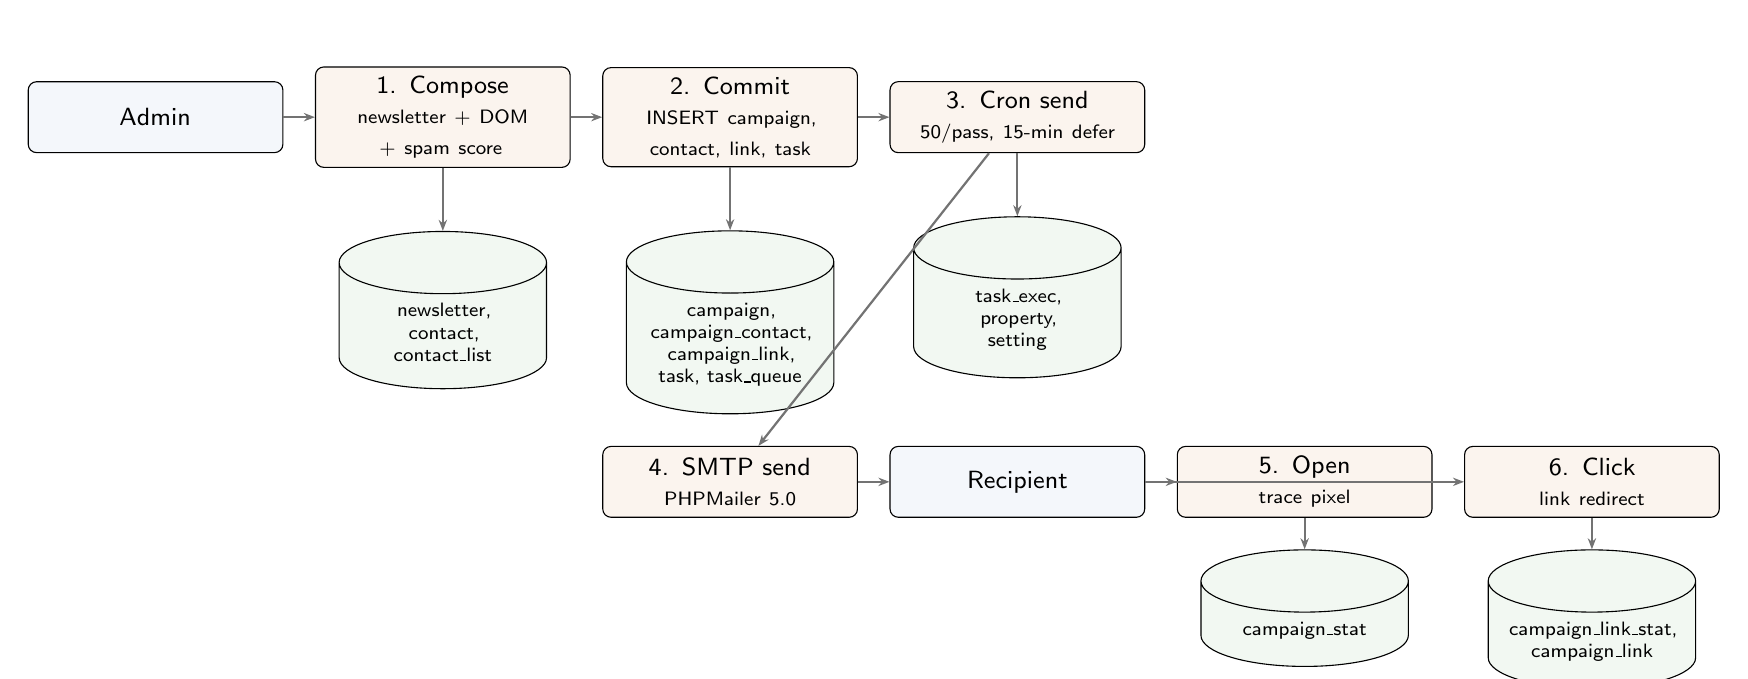
\begin{tikzpicture}[
  box/.style={draw, rounded corners=3pt, text width=3.0cm, minimum height=0.9cm, align=center, font=\small\sffamily, fill=nodefill},
  hotbox/.style={draw, rounded corners=3pt, text width=3.0cm, minimum height=0.9cm, align=center, font=\small\sffamily, fill=nodefillalt},
  db/.style={draw, cylinder, shape border rotate=90, aspect=0.3, text width=2.4cm, minimum height=0.9cm, align=center, font=\scriptsize\sffamily, fill=nodefillgreen},
  arr/.style={-{Stealth[length=4pt]}, thick, black!55}
]
  \node[box] (admin) {Admin};
  \node[hotbox, right=0.4cm of admin] (compose) {1. Compose\\\scriptsize newsletter + DOM + spam score};
  \node[hotbox, right=0.4cm of compose] (commit) {2. Commit\\\scriptsize INSERT campaign, contact, link, task};
  \node[hotbox, right=0.4cm of commit] (cron) {3. Cron send\\\scriptsize 50/pass, 15-min defer};

  \node[db, below=0.8cm of compose] (db1) {newsletter,\\contact,\\contact\_list};
  \node[db, below=0.8cm of commit] (db2) {campaign,\\campaign\_contact,\\campaign\_link,\\task, task\_queue};
  \node[db, below=0.8cm of cron] (db3) {task\_exec,\\property,\\setting};

  \node[hotbox, below=0.4cm of db2] (smtp) {4. SMTP send\\\scriptsize PHPMailer 5.0};
  \node[box, right=0.4cm of smtp] (recipient) {Recipient};
  \node[hotbox, right=0.4cm of recipient] (open) {5. Open\\\scriptsize trace pixel};
  \node[hotbox, right=0.4cm of open] (click) {6. Click\\\scriptsize link redirect};

  \node[db, below=0.4cm of open] (db4) {campaign\_stat};
  \node[db, below=0.4cm of click] (db5) {campaign\_link\_stat,\\campaign\_link};

  \draw[arr] (admin) -- (compose);
  \draw[arr] (compose) -- (commit);
  \draw[arr] (commit) -- (cron);
  \draw[arr] (compose) -- (db1);
  \draw[arr] (commit) -- (db2);
  \draw[arr] (cron) -- (db3);
  \draw[arr] (cron) -- (smtp);
  \draw[arr] (smtp) -- (recipient);
  \draw[arr] (recipient) -- (open);
  \draw[arr] (recipient) -- (click);
  \draw[arr] (open) -- (db4);
  \draw[arr] (click) -- (db5);
\end{tikzpicture}%
}
\caption{The 6-stage campaign pipeline at a glance. Stage 1--2 are
admin-side (compose + commit). Stage 3--4 are cron-side (send +
SMTP). Stage 5--6 are recipient-side (open pixel + click redirect).
The full lifecycle trace is in Section~\ref{sec:trace}.}
\label{fig:overview}
\end{figure}

% ============================================================
\section{The Marketing Database Schema}\label{sec:schema}
% ============================================================

The marketing subsystem uses 9 tables (plus the shared
\texttt{task}, \texttt{task\_queue}, \texttt{task\_exec},
\texttt{property}, and \texttt{setting} tables).

\subsection{The 9 Marketing Tables}

\footnotesize\sloppy
\begin{longtable}{>{\raggedright\arraybackslash}p{3.4cm}p{3.4cm}>{\raggedright\arraybackslash}p{7.5cm}}
\caption{The 9 marketing tables.}\label{tab:marketing-tables}\\
\toprule
\textbf{Table} & \textbf{Primary key} & \textbf{Purpose} \\
\midrule
\endfirsthead
\toprule
\textbf{Table} & \textbf{Primary key} & \textbf{Purpose} \\
\midrule
\endhead
\bottomrule
\endfoot
\texttt{newsletter}             & \texttt{newsletter\_id}        & Reusable email body (name, textbody, htmlbody, status, dates). \\
\texttt{campaign}               & \texttt{campaign\_id}          & A sending of a newsletter (newsletter\_id, name, subject, from\_name, from\_email, replyto\_email, trace\_email, trace\_click, embed\_image, repeat, date\_start, date\_end). \\
\texttt{campaign\_contact}      & \texttt{campaign\_contact\_id} & One recipient of one campaign (campaign\_id, contact\_id, task\_queue\_id, name, email, status). \\
\texttt{campaign\_link}         & \texttt{campaign\_link\_id}    & Trackable link (campaign\_id, url, redirect, link, date\_added). \\
\texttt{campaign\_link\_stat}   & \texttt{...\_stat\_id}         & Link-click event (campaign\_id, contact\_id, customer\_id, link, full HTTP context). \\
\texttt{campaign\_stat}         & \texttt{campaign\_stat\_id}    & Email-open event (campaign\_id, contact\_id, customer\_id, full HTTP context). \\
\texttt{contact}                & \texttt{contact\_id}           & CRM contact (customer\_id, name, email, telephone, provider, is\_active, is\_deleted). \\
\texttt{contact\_list}          & \texttt{contact\_list\_id}     & Named list of contacts (name, description, status, dates). \\
\texttt{contact\_to\_list}      & \texttt{...\_list\_id}         & Junction: contact $\leftrightarrow$ list (unique on (contact\_list\_id, contact\_id)). \\
\end{longtable}

\subsection{Notable Schema Details}

\subsubsection{The \texttt{campaign\_contact.task\_queue\_id} Column}

The schema declares a \texttt{task\_queue\_id} column on
\texttt{campaign\_contact}, suggesting a foreign-key relationship
between a recipient and their queued send task. The source reveals
this column is \emph{never written}. The relationship between a
campaign recipient and their \texttt{task\_queue} row is implicit
(matching \texttt{campaign\_id} + \texttt{contact\_id} in the
queue row's serialised \texttt{params}).

\subsubsection{The \texttt{campaign\_link} Dual-Column URL Storage}

\texttt{campaign\_link} stores two URL columns:

\begin{itemize}[leftmargin=1.6em,itemsep=2pt]
  \item \texttt{url} --- the rewritten tracking URL
        (\texttt{.../link\&...\&link\_index=<md5>}).
  \item \texttt{redirect} --- the original \texttt{href} from the
        newsletter HTML (e.g.\ \texttt{https://shop.example/spring}).
  \item \texttt{link} --- the md5 nonce used as the lookup key.
\end{itemize}

The \texttt{link} redirect endpoint looks up the original URL via
\texttt{SELECT DISTINCT redirect FROM campaign\_link WHERE link =
\$link\_index}. Notably, this lookup is \emph{not} scoped by
\texttt{campaign\_id} --- any campaign's link nonce can be
resolved by any other campaign's redirect handler.

\subsubsection{The Telemetry Tables}

\texttt{campaign\_stat} and \texttt{campaign\_link\_stat} both
record a remarkably rich HTTP context per event:
\texttt{store\_url}, \texttt{server} (serialised
\texttt{\$\_SERVER}), \texttt{session} (serialised
\texttt{\$\_SESSION}), \texttt{request} (serialised
\texttt{\$\_REQUEST}), \texttt{ref} (referrer),
\texttt{browser}, \texttt{browser\_version}, \texttt{os},
\texttt{ip}, \texttt{date\_added}. This is the same forensic
HTTP-context snapshot pattern v1 identified in the
\texttt{stat}, \texttt{search}, and \texttt{user\_activity}
tables.

\subsubsection{The Mailserver Storage Overload}

There is no dedicated \texttt{mailserver} table. Mailserver
credentials are stored in the \texttt{setting} table under group
\texttt{mail\_server}, with the key being a unique ID (e.g.\
\texttt{abc123def4}) and the value being a serialised PHP array
of \texttt{server, port, security, username, password}. The
\texttt{password} is base64-encoded (not encrypted).

Per-campaign mailserver selection is stored in the polymorphic
\texttt{property} EAV table: \texttt{object\_type='campaign'},
\texttt{group='mail\_server'}, \texttt{key='mail\_server\_id'},
\texttt{value=serialize(\$mail\_server\_id)}.

% ============================================================
\section{Newsletter Composition}\label{sec:newsletters}
% ============================================================

A newsletter is a reusable email body. The admin creates one via
\texttt{marketing/newsletter/insert}.

\subsection{The Newsletter Controller}

\texttt{app/admin/controller/marketing/newsletter.php} (794 lines)
handles newsletter CRUD. The \texttt{insert()} method is the most
interesting:

\begin{lstlisting}[caption={\texttt{ControllerMarketingNewsletter::insert()} --- newsletter creation with base64 image extraction (abridged).},label={lst:newsletter-insert}]
public function insert() {
    if (!$this->hasPermission('modify', 'marketing/newsletter')) {
        return $this->forward('error/permission');
    }
    if ($this->request->isPost() && $this->validateForm()) {
        // 1. Parse the htmlbody with DOMDocument
        $dom = new DOMDocument;
        $dom->loadHTML($this->request->post['htmlbody']);

        // 2. Extract base64-encoded images, write them to DIR_IMAGE/data/
        $images = $dom->getElementsByTagName('img');
        foreach ($images as $image) {
            $src = $image->getAttribute('src');
            if (strpos($src, 'data:') === 0 && strpos($src, 'base64,') !== false) {
                list(, $data) = explode('base64,', $src);
                $ext = substr($src, strpos($src, '/') + 1, strpos($src, ';') - strpos($src, '/') - 1);
                $filename = slugify($this->request->post['name']) . '-' . uniqid() . '_' . time() . '.' . $ext;
                file_put_contents(DIR_IMAGE . 'data/' . $filename, base64_decode($data));
                $image->setAttribute('src', HTTP_IMAGE . 'data/' . $filename);
            }
        }

        // 3. htmlentities the result and save
        $this->request->post['htmlbody'] = htmlentities($dom->saveHTML());
        $this->load->model('marketing/newsletter');
        $this->modelNewsletter->add($this->request->post);
        $this->redirect('marketing/newsletter');
    }
    // ... render form ...
}
\end{lstlisting}

The WYSIWYG editor (used in the form) lets the admin paste images
directly, which the browser embeds as \texttt{data:image/...;base64,...}.
The controller extracts these, writes them to
\texttt{DIR\_IMAGE/data/}, and replaces the \texttt{src} with an
HTTP URL. The result is then \texttt{htmlentities}'d and stored.

\subsection{The Personalisation Tokens}

The newsletter HTML body can contain \texttt{\{\%placeholder\%\}}
tokens that are substituted at send time. The cron sender
(\S\ref{sec:cron}) substitutes:

\begin{table}[htbp]
\centering
\caption{The 7 personalisation tokens substituted per recipient.}\label{tab:personalisation}
\small
\begin{tabularx}{\columnwidth}{llX}
\toprule
\textbf{Token} & \textbf{Source} & \textbf{Example} \\
\midrule
\texttt{\{\%contact\_id\%\}}    & \texttt{params['contact\_id']}    & 101 \\
\texttt{\{\%campaign\_id\%\}}   & \texttt{params['campaign\_id']}   & 7 \\
\texttt{\{\%fullname\%\}}       & \texttt{params['name']}           & Alice Smith \\
\texttt{\{\%rif\%\}}            & \texttt{params['rif']}            & J-12345678-9 \\
\texttt{\{\%company\%\}}        & \texttt{params['company']}        & Acme C.A. \\
\texttt{\{\%email\%\}}          & \texttt{params['email']}          & alice@x.com \\
\texttt{\{\%telephone\%\}}      & \texttt{params['telephone']}      & +58 212 555 1212 \\
\bottomrule
\end{tabularx}
\end{table}

Plus the \texttt{prepareTemplate()} method substitutes 13
store-level tokens:

\begin{table}[htbp]
\centering
\caption{The 13 store-level template tokens.}\label{tab:template-tokens}
\footnotesize\sloppy
\begin{tabularx}{\columnwidth}{llX}
\toprule
\textbf{Token} & \textbf{Source} & \textbf{Substitution} \\
\midrule
\texttt{\{\%store\_logo\%\}}       & \texttt{config\_logo} & \texttt{<img src="...">} \\
\texttt{\{\%store\_url\%\}}        & \texttt{HTTP\_HOME} & URL \\
\texttt{\{\%url\_login\%\}}        & \texttt{Url::createUrl('account/login')} & URL \\
\texttt{\{\%store\_owner\%\}}      & \texttt{config\_owner} & string \\
\texttt{\{\%store\_name\%\}}       & \texttt{config\_name} & string \\
\texttt{\{\%store\_rif\%\}}        & \texttt{config\_rif} & string \\
\texttt{\{\%store\_email\%\}}      & \texttt{config\_email} & string \\
\texttt{\{\%store\_telephone\%\}}  & \texttt{config\_telephone} & string \\
\texttt{\{\%store\_address\%\}}    & \texttt{config\_address} & string \\
\texttt{\{\%date\_added\%\}}       & \texttt{date('Y-m-d')} & date \\
\texttt{\{\%ip\%\}}                & \texttt{\$\_SERVER['REMOTE\_ADDR']} & IP \\
\texttt{\{\%qr\_code\_store\%\}}   & \texttt{BarcodeQR} for \texttt{HTTP\_HOME} & \texttt{<img src="cache/<slug>.png">} \\
\texttt{\{\%barcode\_39\_order\_id\%\}} & \texttt{Barcode39} for \texttt{C\_CODE} & \texttt{<img src="cache/<slug>\_barcode\_39.gif">} \\
\bottomrule
\end{tabularx}
\end{table}

A ``Powered By Necotienda <year>'' footer is appended to every
email body.

\subsection{The Model Schema Mismatch}

\begin{findingbox}[Schema mismatch in \texttt{ModelMarketingNewsletter}]
\texttt{app/admin/model/marketing/newsletter.php} (80 lines)
declares \texttt{\$table = 'post'} and \texttt{\$fields} for the
CMS \texttt{post} table, not the \texttt{newsletter} table. The
Model base class's generic CRUD uses these declarations. In
practice, the controller's \texttt{insert()} calls
\texttt{\$this->modelNewsletter->add(\$this->request->post)},
which (via the Model base) would attempt an
\texttt{INSERT INTO post SET ...} with the newsletter fields ---
which would either fail or insert into the wrong table.

The storefront \texttt{app/shop/model/marketing/newsletter.php}
(21 lines) has the same mismatch.

This is a live bug in the source. v4 documents it; it does not
propose a fix.
\end{findingbox}

% ============================================================
\section{Contacts and Contact Lists}\label{sec:contacts}
% ============================================================

A contact is a CRM record (optionally linked to a customer via
\texttt{customer\_id}). A contact list is a named collection.
Contacts and lists are many-to-many via
\texttt{contact\_to\_list}.

\subsection{The Contact Controller}

\texttt{app/admin/controller/marketing/contact.php} (959 lines)
handles contact CRUD plus a 3-step AJAX import wizard and a vCard
export.

\subsubsection{The Import Wizard}

The import is a 3-step AJAX flow:

\begin{enumerate}[leftmargin=1.6em,itemsep=2pt]
  \item Step 1: admin uploads a CSV. The controller parses it,
        caches the parsed rows in \texttt{contact.import.<session>},
        and renders a preview table.
  \item Step 2: admin maps CSV columns to contact fields. The
        mapping is cached.
  \item Step 3: admin confirms. The controller reads the cached
        rows + mapping, inserts new contacts (deduping by email),
        and adds them to the selected contact list.
\end{enumerate}

The cache is keyed by session ID, so multiple admins can run
imports concurrently without colliding.

\subsubsection{The vCard Export}

The vCard export generates a \texttt{.vcf} file for each contact.
Notably, the cleanup step before generation:

\begin{lstlisting}[caption={The vCard export cleanup (abridged).},label={lst:vcard-cleanup}]
// Delete every .vcf in DOCUMENT_ROOT as cleanup
foreach (glob($_SERVER['DOCUMENT_ROOT'] . '/*.vcf') as $file) {
    unlink($file);
}
// Then generate the new .vcf files
foreach ($contacts as $contact) {
    $vcard = new VCard();
    $vcard->addName($contact['lastname'], $contact['firstname']);
    $vcard->addEmail($contact['email']);
    // ...
    file_put_contents($_SERVER['DOCUMENT_ROOT'] . '/' . $contact['slug'] . '.vcf', $vcard);
}
\end{lstlisting}

The cleanup deletes \emph{every} \texttt{.vcf} in the web root
before generating new ones. This is an unusual cleanup strategy.

\subsection{The Contact List Controller}

\texttt{app/admin/controller/marketing/list.php} (579 lines)
handles contact list CRUD. A list has a name, description, and
status. Contacts are added to lists via the
\texttt{contact\_to\_list} junction (unique on
\texttt{(contact\_list\_id, contact\_id)} to prevent duplicates).

\subsection{The \texttt{ModelMarketingList} Type Bug}

\begin{findingbox}[Type bug in \texttt{ModelMarketingList}]
\texttt{app/admin/model/marketing/list.php} declares
\texttt{\$fields['name']} with type \texttt{int}. The
\texttt{contact\_list.name} column is \texttt{VARCHAR(250)}. The
Model base's \texttt{buildSQLQuery} uses the declared type to
cast filter values --- so filtering by name would cast the
search string to int, breaking the query.
\end{findingbox}

% ============================================================
\section{The Campaign Composer and Commit}\label{sec:campaigns}
% ============================================================

A campaign is a sending of a newsletter to a set of contacts. The
admin creates one in two phases: \emph{compose} (preview) and
\emph{commit} (enqueue).

\subsection{Phase 1 --- Compose (\texttt{marketing/campaign/insert})}

\texttt{app/admin/controller/marketing/campaign.php::insert()} (the
compose entry point) does:

\begin{enumerate}[leftmargin=1.6em,itemsep=2pt]
  \item Loads the newsletter by \texttt{newsletter\_id}.
  \item Parses the newsletter HTML with \texttt{DOMDocument}.
  \item If \texttt{embed\_image} is on, embeds each \texttt{<img>}
        as base64.
  \item If \texttt{trace\_email} is on, appends a tracking-pixel
        \texttt{<img>} with
        \texttt{src=Url::createUrl("marketing/campaign/trace",
        ['contact\_id'=>'\{\%contact\_id\%\}',
        'campaign\_id'=>'\{\%campaign\_id\%\}'])}.
  \item If \texttt{trace\_click} is on, iterates \texttt{<a>} tags:
        \begin{itemize}[itemsep=2pt]
          \item Generates \texttt{\$link\_index = md5(time() .
                mt\_rand(1000000,9999999) . \$href)} (a 32-hex-char
                nonce).
          \item Rewrites \texttt{href} to
                \texttt{Url::createUrl("marketing/campaign/link",
                ['contact\_id'=>'\{\%contact\_id\%\}',
                'campaign\_id'=>'\{\%campaign\_id\%\}',
                'link\_index'=>\$link\_index])}.
          \item Collects \texttt{\$links[] = ['url', 'redirect',
                'link\_index']} per link.
        \end{itemize}
  \item Loads the contacts from the selected contact lists:
        \texttt{SELECT *, t.date\_Added AS created, t.email AS mail
        FROM contact t LEFT JOIN customer c ON (c.customer\_id =
        t.customer\_id) LEFT JOIN contact\_to\_list c2l ON
        (t.contact\_id = c2l.contact\_id) WHERE c2l.contact\_list\_id
        IN (5)}.
  \item Deduplicates by email.
  \item Computes \texttt{date\_start\_exec} and
        \texttt{date\_end\_exec} from the POST year/month/day/hour/minute/meridium
        fields.
  \item \texttt{htmlentities(\$dom->saveHTML())} $\to$ \texttt{\$htmlbody}.
  \item \textbf{Spam scoring}: \texttt{require\_once(... 'spam\_rules.php')},
        iterates \texttt{\$spam\_rules}, computes \texttt{\$score} +
        \texttt{\$broken\_rules}.
  \item Caches \texttt{campaign.html.temp} and
        \texttt{campaign.data.temp} (serialised
        \texttt{['to'=>\$to, 'post'=>\$post, 'links'=>\$links]}).
  \item Renders the \texttt{beforeSend} preview page with stats:
        total\_embed\_images, total\_trace\_links, total\_images,
        total\_links, date\_start\_exec, spam\_score, broken\_rules,
        email\_size, contacts count.
\end{enumerate}

\subsection{Phase 2 --- Commit (\texttt{marketing/campaign/send})}

\texttt{ControllerMarketingCampaign::send()} (the commit entry
point, clicked from the beforeSend preview):

\begin{lstlisting}[caption={\texttt{ControllerMarketingCampaign::send()} --- the commit phase (abridged).},label={lst:campaign-commit}]
public function send() {
    // 1. Read the cached composed HTML and data
    $htmlbody = html_entity_decode($this->cache->get("campaign.html.temp"));
    $htmlbody = str_replace('%7B', '{', $htmlbody);  // decode URL-encoded placeholders
    $htmlbody = str_replace('%7D', '}', $htmlbody);
    $data = unserialize($this->cache->get("campaign.data.temp"));
    $to = $data['to'];        // 3 contacts
    $campaign = $data['post'];
    $links = $data['links'];  // 1 link

    // 2. INSERT campaign row
    $campaign['contacts'] = $to;
    $campaign_id = $this->modelCampaign->add($campaign);  // → INSERT INTO campaign ...
    // (the model's on('save') hook inserts campaign_contact rows)

    // 3. Store the mailserver_id in the EAV property table
    $this->modelCampaign->setProperty($campaign_id, 'mail_server', 'mail_server_id', $campaign['mail_server_id']);

    // 4. Build the Task
    $task = new Task($this->registry);
    $task->object_id = $campaign_id;
    $task->object_type = 'campaign';
    $task->task = $campaign['name'];
    $task->type = 'send';
    $task->time_exec = $campaign['date_start_exec'];
    $task->params = ['job' => 'send_campaign', 'campaign_id' => $campaign_id];
    $task->run_once = true;
    $task->status = 1;

    // 5. Per-recipient: substitute body placeholders, cache, and enqueue
    foreach ($to as $sort_order => $contact) {
        // Per-link: substitute {contact_id} and {campaign_id}, INSERT campaign_link
        foreach ($links as $link) {
            $link['url'] = str_replace('{%contact_id%}', $contact['contact_id'], $link['url']);
            $link['url'] = str_replace('{%campaign_id%}', $campaign_id, $link['url']);
            $this->modelCampaign->addLink($link, $campaign_id);
        }
        $params = ['contact_id'=>$contact['contact_id'], 'name'=>$contact['name'],
                   'email'=>$contact['email'], 'campaign_id'=>$campaign_id];
        $queue = ['params'=>$params, 'status'=>1, 'time_exec'=>$campaign['date_start_exec']];
        // Substitute the body-level placeholders
        $htmlbody = str_replace('{%contact_id%}', $contact['contact_id'], $htmlbody);
        $htmlbody = str_replace('{%campaign_id%}', $campaign_id, $htmlbody);
        $ck = "campaign.html.{$campaign_id}.{$contact['contact_id']}";
        $this->cache->set($ck, $htmlbody);
        $task->addQueue($queue);
    }

    // 6. INSERT task + task_queue rows
    $task->createSendTask();
    $this->redirect('marketing/campaign');
}
\end{lstlisting}

\subsection{The Double Link Rewriting}

\begin{findingbox}[Per-recipient link rewriting happens TWICE per campaign]
The compose phase (Phase 1) rewrites every \texttt{<a href>} into
a trackable URL and collects the \texttt{\$links} array. The
commit phase (Phase 2) inserts \texttt{campaign\_link} rows ---
one per recipient per link, all with the \emph{same} \texttt{link}
nonce (because the nonce was generated once in compose).

Then the cron sender (Phase 3, \S\ref{sec:cron}) rewrites the
links \emph{again} --- it generates a \emph{fresh} nonce per
recipient per link and inserts new \texttt{campaign\_link} rows.

The result: each tracked link ends up with \emph{two}
\texttt{campaign\_link} rows per recipient --- one from the commit
phase, one from the cron. The commit-phase rows are effectively
dead data because the cron's fresh nonces are what end up in the
sent email.

If the per-recipient cache \texttt{campaign.html.<cid>.<contact\_id>}
hits, the cron skips the rewriting (and the second
\texttt{campaign\_link} INSERT). So the double-rewriting only
manifests on cache miss.
\end{findingbox}

% ============================================================
\section{The Cron Sender}\label{sec:cron}
% ============================================================

\texttt{system/cron/api/send.php} (511 lines) is the most
important file in the marketing subsystem. The \texttt{CronSend}
class picks up due \texttt{task} rows whose
\texttt{params['job']} is \texttt{send\_campaign},
\texttt{send\_birthday}, or \texttt{send\_recommended\_products},
and dispatches to the matching private method.

\subsection{The \texttt{sendCampaign} Algorithm}

\begin{lstlisting}[caption={\texttt{CronSend::sendCampaign()} --- the campaign sender (abridged).},label={lst:send-campaign}]
public function sendCampaign($task) {
    // 1. Lock check
    if ($this->isLocked('send_campaign', $task->task_id)) {
        $task->addMinute(15);  // defer 15 min
        return;
    }

    // 2. Acquire lock
    $task->start();  // DELETE + INSERT INTO task_exec

    // 3. Load campaign + newsletter
    $query = $this->db->query("SELECT * FROM campaign c
        LEFT JOIN newsletter n ON (n.newsletter_id = c.newsletter_id)
        WHERE campaign_id = '" . (int)$task->params['campaign_id'] . "'");
    $campaign_info = $query->row;

    // 4. Load mailserver config from EAV property + setting tables
    $ms_query = $this->db->query("SELECT * FROM property
        WHERE object_type='campaign' AND group='mail_server'
        AND key='mail_server_id' AND object_id = '" . (int)$task->params['campaign_id'] . "'");
    $mail_server_id = unserialize($ms_query->row['value']);
    $srv_query = $this->db->query("SELECT * FROM setting
        WHERE group='mail_server' AND key='" . $this->db->escape($mail_server_id) . "'");
    $mail_server = unserialize($srv_query->row['value']);
    // $mail_server = ['server'=>'smtp.gmail.com', 'port'=>'587', 'security'=>'tls',
    //                 'username'=>'marketing@shop.example', 'password'=>'app-password']

    // 5. Load newsletter HTML body
    $htmlbody = html_entity_decode($campaign_info['htmlbody']);

    // 6. Per-queue loop (max 50 per pass)
    $count = 0;
    foreach ($task->getTaskQueue() as $key => $queue) {
        if ($count >= 50) break;
        $params = unserialize($queue['params']);

        // 6a. Cache lookup (per-recipient rewritten HTML)
        $cacheKey = "campaign.html.{$params['campaign_id']}.{$params['contact_id']}";
        $cached = $this->cache->get($cacheKey);
        if ($cached) {
            $htmlbody = html_entity_decode($cached);
        } else {
            // 6b. Cache miss: rebuild
            $htmlbody = str_replace("%7B", "{", $htmlbody);
            $htmlbody = str_replace("%7D", "}", $htmlbody);
            $htmlbody = str_replace("{%contact_id%}", $params['contact_id'], $htmlbody);
            $htmlbody = str_replace("{%campaign_id%}", $params['campaign_id'], $htmlbody);
            $htmlbody = str_replace("{%fullname%}", $params['name'], $htmlbody);
            $htmlbody = str_replace("{%rif%}", $params['rif'], $htmlbody);
            $htmlbody = str_replace("{%company%}", $params['company'], $htmlbody);
            $htmlbody = str_replace("{%email%}", $params['email'], $htmlbody);
            $htmlbody = str_replace("{%telephone%}", $params['telephone'], $htmlbody);
            $htmlbody = $this->prepareTemplate($htmlbody, $params);

            // 6c. DOM parse, optional image embedding, tracking pixel, link rewriting
            $dom = new DOMDocument;
            $dom->loadHTML($htmlbody);
            if ($params['embed_image']) { /* base64-embed images */ }
            // Append tracking pixel
            $trace_url = Url::createUrl("marketing/campaign/trace", [...], 'NONSSL', HTTP_HOME);
            $trackEmail = $dom->createElement('img');
            $trackEmail->setAttribute('src', $trace_url);
            $dom->appendChild($trackEmail);
            // Rewrite every <a href> with a fresh nonce, INSERT campaign_link
            foreach ($dom->getElementsByTagName('a') as $link) {
                $href = $link->getAttribute('href');
                if (empty($href) || $href == "#" || strpos($href, "mailto:") !== false) continue;
                $link_index = md5(time() . mt_rand(1000000, 9999999) . $href);
                $_link = Url::createUrl("marketing/campaign/link", [...], 'NONSSL', HTTP_HOME);
                $this->db->query("INSERT INTO campaign_link SET campaign_id=..., url=..., redirect=..., link=..., date_added=NOW()");
                $link->setAttribute('href', $_link);
            }
            $htmlbody = $dom->saveHTML();
        }

        // 7. Send via PHPMailer 5.0
        $mailer = new Mailer();
        $mailer->IsSMTP();
        $mailer->Host = $mail_server['server'];
        $mailer->Port = $mail_server['port'];
        $mailer->SMTPSecure = $mail_server['security'];
        $mailer->Username = $mail_server['username'];
        $mailer->Password = base64_decode($mail_server['password']);
        $mailer->SMTPAuth = true;
        $mailer->AddAddress($params['email'], $params['name']);
        $mailer->IsHTML(true);
        $mailer->SetFrom($campaign_info['from_email'], $campaign_info['from_name']);
        $mailer->AddReplyTo($campaign_info['replyto_email'], $campaign_info['from_name']);
        $mailer->Subject = $campaign_info['subject'];
        $mailer->Body = $htmlbody;
        $mailer->Send();
        $mailer->ClearAllRecipients();

        // 8. Mark queue entry done
        $task->setQueueDone($key);
        $count++;
    }

    // 9. End-of-loop: defer or complete
    if (count($task->getTaskDos($task->task_id)) > 0) {
        $task->addMinute(15);  // more pending, defer 15 min
    } else {
        $task->setTaskDone();  // all done
    }
    $task->update();
}
\end{lstlisting}

\subsection{The Locking Mechanism}

The lock is implemented via the \texttt{task\_exec} table
(MyISAM has no row-level locks, so the application uses
delete-then-insert as a best-effort lock):

\begin{lstlisting}[caption={\texttt{CronSend::isLocked()} --- the lock check.},label={lst:is-locked}]
private function isLocked($job, $current_task_id) {
    $query = $this->db->query("SELECT * FROM task_exec WHERE type = '" . $this->db->escape($job) . "'");
    if (count($query->rows)) {
        $queue = $this->db->query("SELECT COUNT(*) AS total FROM task_queue
            WHERE status = '1' AND task_id = '" . (int)$query->row['task_id'] . "'");
        if ($queue->row['total'] > 0) {
            if ($current_task_id == $query->row['task_id']) {
                return false;       // I already hold the lock
            } else {
                return true;        // someone else holds it
            }
        } else {
            // Stale lock, clear it
            $this->db->query("DELETE FROM task_exec WHERE type = '" . $this->db->escape($job) . "'");
            return false;
        }
    }
    return false;
}
\end{lstlisting}

\subsection{The 50-Email Throttle}

The sender processes at most 50 queue entries per pass. If the
queue is not empty after 50 sends, the task is deferred 15 minutes
(\texttt{\$task->addMinute(15)}), and the next cron tick picks it
up. So a 1,000-recipient campaign takes
$\lceil 1000/50 \rceil = 20$ passes, or roughly 5 hours at a
15-minute cron interval. This throttle is hard-coded; there is no
per-mailserver rate-limit configuration.

\subsection{The Per-Pass Cache}

The per-recipient rewritten HTML is cached at
\texttt{campaign.html.<campaign\_id>.<contact\_id>}. The commit
phase (Phase 2) populates this cache. The cron sender reads it.
On a cache hit, the cron skips the DOM parse, the personalisation
substitution, the image embedding, the tracking-pixel append, and
the link rewriting --- it just sends the cached HTML. On a cache
miss (e.g.\ if the cache was cleared), the cron rebuilds
everything, which is where the double link rewriting manifests.

% ============================================================
\section{The Tracking Endpoints}\label{sec:tracking}
% ============================================================

The storefront has two endpoints that record recipient
interactions: \texttt{trace} (email open) and \texttt{link} (link
click).

\subsection{The Tracking Pixel (\texttt{marketing/campaign/trace})}

\begin{lstlisting}[caption={\texttt{ControllerMarketingCampaign::trace()} --- the open-tracking pixel.},label={lst:trace}]
public function trace() {
    header('Cache-Control: no-cache');
    header('Content-type: image/jpeg');
    if ($this->request->hasQuery('campaign_id')) {
        $this->load->model('marketing/campaign');
        $this->modelCampaign->trackEmail(
            $this->request->getQuery('campaign_id'),
            $this->request->getQuery('contact_id')
        );
        if ($this->request->hasQuery('sendCampaign')) {
            $this->link2Campaign($this->request->getQuery('sendCampaign'));
        }
    }
    readfile('https://necoyoad.com/.../firma_necoyoad.jpg');
}
\end{lstlisting}

The endpoint:

\begin{enumerate}[leftmargin=1.6em,itemsep=2pt]
  \item Sets \texttt{Cache-Control: no-cache} and
        \texttt{Content-type: image/jpeg} (so the email client
        treats the response as an image).
  \item Calls \texttt{trackEmail()}, which INSERTs a
        \texttt{campaign\_stat} row with the campaign\_id,
        contact\_id, customer\_id (if logged in), and the full
        HTTP context (serialised \texttt{\$\_SERVER},
        \texttt{\$\_SESSION}, \texttt{\$\_REQUEST}, referrer,
        browser, OS, IP).
  \item If \texttt{sendCampaign} query param is present, calls
        \texttt{link2Campaign()} (a hidden follow-up-campaign
        trigger, \S\ref{sec:aux-tasks}).
  \item Streams a 1x1 JPEG from \texttt{necoyoad.com} ---
        \texttt{readfile(...)} the pixel image.
\end{enumerate}

\begin{findingbox}[The tracking pixel is hard-coded to a Necoyoad-CDN image]
The tracking pixel image is fetched from a hard-coded URL on the
Necoyoad marketing site
(\texttt{necoyoad.com/.../firma\_necoyoad.jpg}), not the local
store. This means every tracking-pixel request makes an outbound
HTTP call to \texttt{necoyoad.com}. If the Necoyoad marketing site
is down, the tracking still records the open (the
\texttt{campaign\_stat} INSERT happens before the
\texttt{readfile}), but the recipient's email client shows a
broken image icon.
\end{findingbox}

\subsection{The Link Redirect (\texttt{marketing/campaign/link})}

\begin{lstlisting}[caption={\texttt{ControllerMarketingCampaign::link()} --- the click-tracking redirect.},label={lst:link}]
public function link() {
    if ($this->request->hasQuery('campaign_id')) {
        $this->load->model('marketing/campaign');
        $this->modelCampaign->trackLink(
            $this->request->getQuery('campaign_id'),
            $this->request->getQuery('contact_id'),
            $this->request->getQuery('link_index')
        );
        if ($this->request->hasQuery('sendCampaign')) {
            $this->link2Campaign($this->request->getQuery('sendCampaign'));
        }
        $link_index = $this->request->getQuery('link_index');
        $redirectTo = $this->modelCampaign->getLink($link_index);
        if ($redirectTo) {
            $this->redirect($redirectTo);
        } else {
            $this->redirect(HTTP_HOME);
        }
    }
}
\end{lstlisting}

The endpoint:

\begin{enumerate}[leftmargin=1.6em,itemsep=2pt]
  \item Calls \texttt{trackLink()}, which INSERTs a
        \texttt{campaign\_link\_stat} row with the campaign\_id,
        contact\_id, customer\_id, the link nonce, and the full
        HTTP context.
  \item If \texttt{sendCampaign} query param is present, calls
        \texttt{link2Campaign()}.
  \item Looks up the original URL via \texttt{getLink()}:
        \texttt{SELECT DISTINCT redirect FROM campaign\_link WHERE
        link = \$link\_index}.
  \item 302-redirects to the original URL (or to \texttt{HTTP\_HOME}
        if not found).
\end{enumerate}

\begin{findingbox}[The \texttt{campaign\_link} lookup is not scoped by \texttt{campaign\_id}]
\texttt{getLink(\$link)} does \texttt{SELECT DISTINCT redirect
FROM campaign\_link WHERE link = \$link}. The lookup is by nonce
only, not by \texttt{campaign\_id}. This means a nonce from one
campaign can resolve to a redirect from a different campaign
(if the nonces collide, which is unlikely with md5 but not
impossible). It also means the lookup returns the first matching
row, which (per the double-rewriting finding) could be either
the commit-phase row or the cron-phase row --- but since both
have the same \texttt{redirect} value, the result is correct.
\end{findingbox}

\subsection{The \texttt{trackEmail} SQL Bug}

\begin{findingbox}[\texttt{trackEmail} and \texttt{trackLink} use \texttt{INSERT} not \texttt{INSERT INTO}]
The \texttt{ModelMarketingCampaign::trackEmail()} and
\texttt{trackLink()} methods use \texttt{INSERT <table> SET ...}
instead of the standard \texttt{INSERT INTO <table> SET ...}.
MySQL tolerates \texttt{INSERT} as a synonym for \texttt{INSERT
INTO}, so this works in practice, but it is non-standard SQL and
would fail on strict SQL modes or other databases.
\end{findingbox}

% ============================================================
\section{The Mailer (PHPMailer 5.0)}\label{sec:mailer}
% ============================================================

The campaign sender uses \texttt{system/library/email/mailer.php}
(2,289 lines), which is PHPMailer 5.0 (released 2009) with the
class renamed from \texttt{PHPMailer} to \texttt{Mailer}.

\subsection{Two Parallel Mailers}

\begin{findingbox}[Two parallel hand-rolled mailers coexist]
The codebase has two parallel mailer stacks:

\begin{itemize}[leftmargin=1.6em,itemsep=2pt]
  \item \texttt{system/library/email/mailer.php} (2,289 lines) ---
        PHPMailer 5.0, class \texttt{Mailer}. Used by the cron
        sender for campaigns.
  \item \texttt{system/library/mail.php} (397 lines) --- a
        separate, simpler \texttt{Mail} class. Used by the
        order-confirmation email flow (\texttt{checkout/success}).
  \item \texttt{system/library/ntsmailer.php} (164 lines) ---
        \texttt{ntsMailer}, a thin wrapper that picks between the
        two based on config.
\end{itemize}

Different parts of the codebase use different mailers. The
campaign subsystem always uses \texttt{Mailer} (PHPMailer 5.0).
\end{findingbox}

\subsection{The SMTP Client}

\texttt{system/library/email/smtp.php} (814 lines) is a
from-scratch SMTP client (not a wrapper around PHP's
\texttt{mail()} or a third-party library). It supports:

\begin{itemize}[leftmargin=1.6em,itemsep=2pt]
  \item \texttt{AUTH LOGIN} (base64-encoded username and password).
  \item \texttt{STARTTLS} (for \texttt{SMTPSecure = 'tls'}).
  \item \texttt{SMTPS} (for \texttt{SMTPSecure = 'ssl'}).
  \item Multiple recipients, CC, BCC, attachments, embedded
        images.
\end{itemize}

It does \emph{not} support \texttt{AUTH CRAM-MD5},
\texttt{AUTH PLAIN}, or \texttt{AUTH XOAUTH2}. So campaigns can
only be sent via SMTP servers that accept \texttt{AUTH LOGIN}
with a username+password (e.g.\ Gmail with an app password, but
not Gmail with OAuth).

\subsection{The POP3 Client (for Bounce)}

\texttt{system/library/email/pop3.php} (406 lines) is a
from-scratch POP3 client. It is used by the (vestigial) bounce
processor (\S\ref{sec:bounce}).

\subsection{The Password Storage}

Mailserver passwords are stored in the \texttt{setting} table,
base64-encoded (not encrypted). The cron sender decodes them with
\texttt{base64\_decode(\$mail\_server['password'])} before passing
to \texttt{Mailer}. This is encoding, not encryption --- anyone
with database read access has all mailserver credentials.

% ============================================================
\section{The Vestigial Bounce Processor}\label{sec:bounce}
% ============================================================

\begin{findingbox}[Bounce processing is entirely vestigial]
\texttt{system/cron/api/bounce.php} (167 lines) is \textbf{not
loaded} by \texttt{cron.php} --- the \texttt{require\_once} for
\texttt{bounce.php} is commented out at line 17. The file's
contents reference \texttt{SENDSTUDIO\_TABLEPREFIX},
\texttt{SENDSTUDIO\_API\_DIRECTORY}, \texttt{Jobs\_Bounce\_API},
\texttt{Jobs\_API}, \texttt{CheckCronSchedule}, \texttt{GetLang},
\texttt{common.php} --- none of which exist in the Necoyoad
codebase. It is a verbatim copy of Interspire SendStudio's
\texttt{admin/cron/bounce.php} and is effectively dead code. It
would fatal-error on \texttt{require\_once dirname(\_\_FILE\_\_) .
'/common.php'} (which doesn't exist).

The function \texttt{Cron\_BounceProcess} (lines 44--165) is a
docstring-only description of the bounce-processing flow it
would perform if the Interspire API were present.
\end{findingbox}

The admin-side \texttt{app/admin/model/marketing/bounce.php}
(194 lines) targets a non-existent \texttt{email\_lists} schema
(another Interspire relic). It defines methods like
\texttt{getBounces()}, \texttt{deleteBounce()},
\texttt{processBounce()} --- but the tables they query
(\texttt{email\_lists}, \texttt{email\_list\_subscriptions},
\texttt{email\_queue}) do not exist in the Necoyoad schema.

The platform has \emph{no working bounce detection}. Bounced
emails are not automatically unsubscribed; the contact stays
active and will be emailed again on the next campaign. The only
way to stop sending to a bounced address is for the admin to
manually mark the contact as \texttt{is\_deleted} or
\texttt{is\_active = 0}.

% ============================================================
\section{The Auxiliary Tasks: Birthday, Promoter, Seller}\label{sec:aux-tasks}
% ============================================================

The cron dispatches three other marketing-related tasks alongside
\texttt{send\_campaign}.

\subsection{\texttt{CronBirthday} (\texttt{system/cron/api/birthday.php}, 97 lines)}

Sends birthday greeting emails. The cron queries
\texttt{SELECT * FROM customer WHERE birthday = TODAY() AND
congrats = 1}, loads the newsletter specified by the
\texttt{marketing\_mailserver\_happy\_birthday} config key, and
for each birthday customer, substitutes
\texttt{\{\%fullname\%\}}, \texttt{\{\%rif\%\}},
\texttt{\{\%company\%\}}, \texttt{\{\%email\%\}},
\texttt{\{\%telephone\%\}} and sends via \texttt{Mailer}.

\begin{findingbox}[Birthday congrats-reset has an AND/OR semantic bug]
After sending, the cron sets \texttt{customer.congrats = 0} to
prevent re-sending next year. The query is:
\texttt{UPDATE customer SET congrats = 0 WHERE customer\_id = X
AND congrats = 1 OR customer\_id = X}. Due to operator
precedence (\texttt{AND} binds tighter than \texttt{OR}), this
parses as \texttt{(customer\_id = X AND congrats = 1) OR
(customer\_id = X)} --- which simplifies to
\texttt{customer\_id = X}. So the update sets
\texttt{congrats = 0} for the customer regardless of the current
value. This happens to be the desired behaviour (always reset),
but the intent was clearly to only reset if currently 1.
\end{findingbox}

\subsection{\texttt{CronPromoter} (\texttt{system/cron/api/promoter.php}, 167 lines)}

Sends ``promoter'' emails --- product recommendations based on
the customer's referral activity. Queries the \texttt{stat} table
for today's product views, picks the top N, and sends a
``recommended products'' email to each promoter (customer with
\texttt{referenced\_by > 0}).

\subsection{\texttt{CronSeller} (\texttt{system/cron/api/seller.php}, 92 lines)}

\begin{findingbox}[\texttt{CronSeller} is a stub]
\texttt{CronSeller} is a stub. The \texttt{run()} method is
empty. It would fatal-error if instantiated (it references
undefined properties) or never be instantiated (the cron
constructor does not instantiate it).
\end{findingbox}

\subsection{\texttt{CronUpdate} (\texttt{system/cron/api/update.php}, 214 lines)}

\begin{findingbox}[\texttt{CronUpdate} is a stub]
\texttt{CronUpdate} is also a stub. It is not instantiated by
the cron constructor. Its \texttt{run()} method contains
commented-out logic for updating campaign statuses (marking
completed campaigns, advancing scheduled ones).
\end{findingbox}

\subsection{The Hidden \texttt{link2Campaign} Mechanism}

The storefront tracking endpoints (\texttt{trace} and
\texttt{link}) have a hidden \texttt{sendCampaign} query
parameter. If present, the endpoint calls
\texttt{link2Campaign(\$campaign\_id)}, which:

\begin{enumerate}[leftmargin=1.6em,itemsep=2pt]
  \item Loads the contact and the source campaign.
  \item Copies the campaign with name suffix \texttt{" - Campaign
        Triggered"}, sets \texttt{date\_start} to
        \texttt{now + 15 minutes} and \texttt{date\_end} to
        \texttt{now + 2 days}, sets \texttt{repeat = ""}.
  \item Targets only the current contact.
  \item Mirrors the \texttt{ControllerMarketingCampaign::send}
        logic: \texttt{modelCampaign->add} + \texttt{setProperty}
        + new \texttt{Task} + \texttt{addQueue} +
        \texttt{createSendTask}.
\end{enumerate}

This is a follow-up-campaign trigger: when a recipient opens (or
clicks) a campaign, a follow-up campaign can be automatically
scheduled for them 15 minutes later. No admin UI exposes this
mechanism --- it would have to be triggered by manually crafting
a URL with \texttt{?sendCampaign=<id>}. It could be used for
forward-to-a-friend (the recipient forwards the email, the
friend's open triggers a follow-up campaign), but no such feature
is implemented.

% ============================================================
\section{The Spam Rules}\label{sec:spam}
% ============================================================

\texttt{system/library/email/spam\_rules.php} (1,177 lines) is a
content-scoring system applied to the campaign HTML body at
compose time. It returns a numeric score and a list of broken
rules.

\subsection{The Three-Layer Spam Pipeline}

\begin{findingbox}[Three layers of spam-rule application]
The spam rules are applied in three layers:

\begin{enumerate}[leftmargin=1.6em,itemsep=2pt]
  \item \texttt{spam\_rules.php} defines a global
        \texttt{\$spam\_rules} array of rule definitions (each
        with a regex/pattern, a score, and a description).
  \item The campaign composer (\texttt{insert()}) iterates
        \texttt{\$spam\_rules}, applies each rule to the HTML
        body, and accumulates \texttt{\$score} +
        \texttt{\$broken\_rules}.
  \item The beforeSend preview displays the score and the broken
        rules, so the admin can see if the email is likely to be
        flagged as spam.
\end{enumerate}

The rules themselves are a mix of content checks (e.g.\ ``too
many exclamation marks'', ``all-caps subject'', ``spammy words
like FREE, GUARANTEE, ACT NOW'') and structural checks (e.g.\
``image-to-text ratio too high'', ``too many colours'',
``javascript present'').
\end{findingbox}

\subsection{The Rule Format}

Each rule in \texttt{\$spam\_rules} is an array with:

\begin{itemize}[leftmargin=1.6em,itemsep=2pt]
  \item \texttt{pattern} --- a regex or string to match.
  \item \texttt{score} --- the numeric penalty if matched.
  \item \texttt{description} --- a human-readable explanation.
  \item \texttt{category} --- e.g.\ \texttt{content},
        \texttt{structure}, \texttt{subject}.
\end{itemize}

The total score is the sum of all matched rules' scores. A score
above a threshold (configurable) is flagged as ``likely spam''.
The admin can still send the campaign, but they are warned.

% ============================================================
\section{The Admin API Marketing Endpoints}\label{sec:api}
% ============================================================

The admin API v1.0.0 has 5 marketing resource endpoints (each
with a paired \texttt{\_data.php} file), following the same
pseudo-REST shape as the other API endpoints (v2 \S7).

\subsection{The 5 Endpoints}

\begin{table}[htbp]
\centering
\caption{The 5 admin API v1.0.0 marketing endpoints.}\label{tab:api-marketing}
\small
\begin{tabularx}{\columnwidth}{llX}
\toprule
\textbf{Resource} & \textbf{Files} & \textbf{Operations} \\
\midrule
\texttt{campaigns}     & \texttt{campaigns.php} (154) + \texttt{\_data.php} (42) & GET (list with filters), POST (create), PUT (update), DELETE. \\
\texttt{contacts}      & \texttt{contacts.php} (151) + \texttt{\_data.php} (32) & Same. \\
\texttt{contact\_lists}& \texttt{contact\_lists.php} (149) + \texttt{\_data.php} (31) & Same. \\
\texttt{mailservers}   & \texttt{mailservers.php} (102) + \texttt{\_data.php} (34) & Same. \\
\texttt{newsletters}   & \texttt{newsletters.php} (147) + \texttt{\_data.php} (32) & Same. \\
\bottomrule
\end{tabularx}
\end{table}

\subsection{The Broken PUT Branches}

\begin{findingbox}[All 5 marketing API PUT branches are broken in different ways]
The PUT (update) branches of all 5 marketing API endpoints are
broken:

\begin{itemize}[leftmargin=1.6em,itemsep=2pt]
  \item \texttt{campaigns.php} PUT: uses the loaded DB row as the
        data source instead of the JSON body.
  \item \texttt{contacts.php} PUT: same.
  \item \texttt{contact\_lists.php} PUT: same.
  \item \texttt{mailservers.php} PUT: references an undefined
        \texttt{\$query} variable (would fatal).
  \item \texttt{newsletters.php} PUT: same as campaigns.
\end{itemize}

The GET, POST, and DELETE branches work. Only PUT is broken. The
\texttt{prepareData()} call in each PUT branch receives the
existing DB row instead of \texttt{\$this->request->post}, so
the update is a no-op (or, for mailservers, a fatal).
\end{findingbox}

% ============================================================
\section{The Campaign Lifecycle Trace}\label{sec:trace}
% ============================================================

This trace walks through a single campaign lifecycle: the admin
creates a newsletter, creates a campaign targeting 3 contacts,
the cron sends it, one recipient opens it, and that recipient
clicks the link.

\subsection{Stage 1 --- Newsletter Create}

\textbf{Entry:} \texttt{POST /admin/index.php?r=marketing/newsletter/insert}
with \texttt{name="Spring Sale"},
\texttt{htmlbody="<html><body><h1>Hi \{\%fullname\%\}</h1><p>Welcome \{\%email\%\}</p><a href='https://shop.example/spring'>Shop now</a></body></html>"}.

\begin{enumerate}[leftmargin=1.6em,itemsep=2pt]
  \item \texttt{ControllerMarketingNewsletter::insert()}.
  \item Permission check: \texttt{hasPermission('modify',
        'marketing/newsletter')}.
  \item Parse \texttt{htmlbody} with \texttt{DOMDocument}.
  \item Iterate \texttt{<img>} tags: none have base64
        \texttt{src}, skip.
  \item \texttt{htmlentities(\$dom->saveHTML())} $\to$
        \texttt{post['htmlbody']}.
  \item \texttt{modelNewsletter->add(\$post)} $\to$
        \texttt{INSERT INTO newsletter SET name='Spring Sale',
        textbody='', htmlbody=..., date\_added=NOW(),
        date\_modified=NOW(), status=1}. Returns
        \texttt{newsletter\_id = 42}.
\end{enumerate}

\textbf{DB writes:} \texttt{newsletter} (1 row).

\subsection{Stage 2 --- Campaign Compose}

\textbf{Entry:} \texttt{POST /admin/index.php?r=marketing/campaign/insert}
with \texttt{name="April Spring Blast", newsletter\_id=42,
subject="Spring Sale Now On", from\_name="NecoShop",
from\_email="marketing@shop.example",
replyto\_email="reply@shop.example", contact\_list=5,
mail\_server\_id="abc123def4", trace\_email=1, trace\_click=1,
embed\_image=0, schedule=2025-04-15 10:00 AM}.

\begin{enumerate}[leftmargin=1.6em,itemsep=2pt]
  \item \texttt{ControllerMarketingCampaign::insert()}.
  \item Load newsletter 42: \texttt{SELECT * FROM newsletter
        WHERE newsletter\_id = 42}.
  \item Parse HTML with \texttt{DOMDocument}.
  \item \texttt{trace\_email=1} $\to$ append tracking-pixel
        \texttt{<img src=".../trace?contact\_id=\{\%contact\_id\%\}\&...">}.
  \item \texttt{trace\_click=1} $\to$ rewrite \texttt{<a href>}:
        \begin{itemize}[itemsep=2pt]
          \item \texttt{\$link\_index = md5(time() . mt\_rand(1000000,9999999) . 'https://shop.example/spring')}
                $\to$ e.g.\ \texttt{a1b2c3d4e5f6...}.
          \item Rewrite \texttt{href} to
                \texttt{.../link?contact\_id=\{\%contact\_id\%\}\&...\&link\_index=<nonce>}.
          \item Collect a \texttt{\$links} entry with the rewritten
                \texttt{url}, the original \texttt{redirect}, and the
                \texttt{link\_index} nonce.
        \end{itemize}
  \item Load contacts from list 5: \texttt{SELECT *, t.date\_Added
        AS created, t.email AS mail FROM contact t LEFT JOIN
        customer c ON (...) LEFT JOIN contact\_to\_list c2l ON
        (...) WHERE c2l.contact\_list\_id IN (5)}. Returns 3
        contacts: Alice (101), Bob (102), Carol (103).
  \item Spam scoring: iterate \texttt{\$spam\_rules}, compute
        \texttt{\$score = 0.5}, \texttt{\$broken\_rules = []}
        (low score, no broken rules).
  \item Cache: \texttt{campaign.html.temp = htmlentities(\$dom->saveHTML())},
        \texttt{campaign.data.temp = serialize(['to'=>\$to, 'post'=>\$post, 'links'=>\$links])}.
  \item Render \texttt{beforeSend} preview with stats.
\end{enumerate}

\textbf{DB reads:} \texttt{newsletter} (1), \texttt{contact} +
\texttt{contact\_to\_list} + \texttt{customer} (1 JOIN).
\textbf{Cache writes:} \texttt{campaign.html.temp},
\texttt{campaign.data.temp}.

\subsection{Stage 3 --- Campaign Commit}

\textbf{Entry:} \texttt{POST /admin/index.php?r=marketing/campaign/send}
(clicked from the beforeSend preview).

\begin{enumerate}[leftmargin=1.6em,itemsep=2pt]
  \item \texttt{ControllerMarketingCampaign::send()}.
  \item Read cache: \texttt{\$htmlbody =
        html\_entity\_decode(cache.get("campaign.html.temp"))}.
        Decode \texttt{\%7B/\%7D} $\to$ \texttt{\{/\}}.
  \item \texttt{\$data = unserialize(cache.get("campaign.data.temp"))}.
        \texttt{\$to = [Alice, Bob, Carol]},
        \texttt{\$links = [spring\_link]}.
  \item \texttt{campaign\_id = modelCampaign->add(\$campaign)}
        $\to$ \texttt{INSERT INTO campaign SET newsletter\_id=42,
        name='April Spring Blast', subject=..., from\_name=...,
        trace\_email=1, trace\_click=1, embed\_image=0,
        date\_start='2025-04-15 10:00:00', ...}. Returns
        \texttt{campaign\_id = 7}.
  \item The model's \texttt{on('save')} hook fires
        \texttt{setContacts(7, \$to)} $\to$
        \texttt{DELETE FROM campaign\_contact WHERE campaign\_id=7}
        then \texttt{INSERT INTO campaign\_contact SET
        campaign\_id=7, contact\_id=101, name='Alice',
        email='alice@x.com', status=1} $\times$ 3.
  \item \texttt{modelCampaign->setProperty(7, 'mail\_server',
        'mail\_server\_id', 'abc123def4')} $\to$
        \texttt{DELETE FROM property WHERE ...} then
        \texttt{INSERT INTO property SET object\_type='campaign',
        object\_id=7, group='mail\_server',
        key='mail\_server\_id', value=serialize('abc123def4')}.
  \item Build \texttt{Task}: \texttt{object\_id=7,
        object\_type='campaign', task='April Spring Blast',
        type='send', time\_exec='2025-04-15 10:00:00',
        params=['job'=>'send\_campaign', 'campaign\_id'=>7],
        run\_once=1, status=1}.
  \item Per recipient (Alice):
        \begin{itemize}[itemsep=2pt]
          \item Per link: \texttt{str\_replace('\{\%contact\_id\%\}', 101, \$link['url'])},
                \texttt{str\_replace('\{\%campaign\_id\%\}', 7, \$link['url'])},
                then \texttt{modelCampaign->addLink(\$link, 7)}
                $\to$ \texttt{INSERT INTO campaign\_link SET
                campaign\_id=7, url='.../link?contact\_id=101\&...',
                redirect='https://shop.example/spring',
                link='<nonce>', date\_added=NOW()}.
          \item \texttt{str\_replace('\{\%contact\_id\%\}', 101, \$htmlbody)},
                \texttt{str\_replace('\{\%campaign\_id\%\}', 7, \$htmlbody)}.
          \item \texttt{cache.set("campaign.html.7.101", \$htmlbody)}.
          \item \texttt{task->addQueue(['params'=>['contact\_id'=>101,
                'name'=>'Alice', 'email'=>'alice@x.com',
                'campaign\_id'=>7], 'status'=>1,
                'time\_exec'=>'2025-04-15 10:00:00'])}.
        \end{itemize}
  \item Same for Bob (102) and Carol (103).
  \item \texttt{task->createSendTask()} $\to$
        \texttt{INSERT INTO task SET store\_id=0, object\_id=7,
        object\_type='campaign', task='April Spring Blast',
        type='send', params=serialize(['job'=>'send\_campaign',
        'campaign\_id'=>7]), time\_exec='2025-04-15 10:00:00',
        run\_once=1, status=1}. Returns \texttt{task\_id = 99}.
  \item Per queue entry: \texttt{INSERT INTO task\_queue SET
        task\_id=99, params=serialize(['contact\_id'=>101, ...]),
        time\_exec='2025-04-15 10:00:00', status=1, sort\_order=0}
        $\times$ 3.
\end{enumerate}

\textbf{DB writes:} \texttt{campaign} (1),
\texttt{campaign\_contact} (3), \texttt{campaign\_link} (3 --- one
per recipient, same nonce), \texttt{property} (1), \texttt{task}
(1), \texttt{task\_queue} (3). \textbf{Cache writes:}
\texttt{campaign.html.7.101}, \texttt{.102}, \texttt{.103}.

\subsection{Stage 4 --- Cron Send}

\textbf{Entry:} \texttt{php /path/to/system/cron/cron.php} (run
by system crontab at 10:00).

\begin{enumerate}[leftmargin=1.6em,itemsep=2pt]
  \item \texttt{Cron::\_\_construct()}: bootstrap, load
        \texttt{setting} for \texttt{store\_id=0}, init mailer.
  \item \texttt{SELECT * FROM task WHERE date\_start\_exec <= NOW()
        AND time\_exec <= NOW() AND status=1 ORDER BY sort\_order
        ASC, time\_exec ASC}. Returns task 99.
  \item \texttt{SELECT * FROM task\_queue WHERE task\_id=99 AND
        status=1 ORDER BY sort\_order ASC, time\_exec ASC}.
        Returns 3 rows.
  \item Hydrate \texttt{Task} object with queue.
  \item \texttt{CronSend::run([task 99])} $\to$
        \texttt{sendCampaign(task 99)}.
  \item \texttt{isLocked('send\_campaign', 99)} $\to$
        \texttt{SELECT * FROM task\_exec WHERE
        type='send\_campaign'} $\to$ no rows $\to$ return false.
  \item \texttt{task->start()} $\to$ \texttt{DELETE FROM
        task\_exec WHERE type='send\_campaign'},
        \texttt{INSERT INTO task\_exec SET task\_id=99,
        type='send\_campaign', status=1, date\_added=NOW()}.
  \item \texttt{SELECT * FROM campaign c LEFT JOIN newsletter n
        ON (...) WHERE campaign\_id=7} $\to$ campaign + newsletter
        row.
  \item \texttt{SELECT * FROM property WHERE
        object\_type='campaign' AND group='mail\_server' AND
        key='mail\_server\_id' AND object\_id=7} $\to$
        \texttt{value='s:10:"abc123def4";'}.
  \item \texttt{\$mail\_server\_id = unserialize(...) = 'abc123def4'}.
  \item \texttt{SELECT * FROM setting WHERE group='mail\_server'
        AND key='abc123def4'} $\to$
        \texttt{value=serialize(['server'=>'smtp.gmail.com',
        'port'=>'587', 'security'=>'tls',
        'username'=>'marketing@shop.example',
        'password'=>base64('app-password')])}.
  \item Per queue entry (Alice, contact\_id=101):
        \begin{itemize}[itemsep=2pt]
          \item \texttt{\$cached = cache.get("campaign.html.7.101")}
                $\to$ HIT. \texttt{\$htmlbody =
                html\_entity\_decode(\$cached)}.
          \item Build \texttt{Mailer}: \texttt{IsSMTP()},
                \texttt{Host='smtp.gmail.com'},
                \texttt{Port=587}, \texttt{SMTPSecure='tls'},
                \texttt{Username='marketing@shop.example'},
                \texttt{Password=base64\_decode('app-password')},
                \texttt{SMTPAuth=true}.
          \item \texttt{AddAddress('alice@x.com', 'Alice')},
                \texttt{IsHTML(true)},
                \texttt{SetFrom('marketing@shop.example', 'NecoShop')},
                \texttt{AddReplyTo('reply@shop.example', 'NecoShop')},
                \texttt{Subject='Spring Sale Now On'},
                \texttt{Body=\$htmlbody}.
          \item \texttt{Send()} $\to$ SMTP to
                \texttt{smtp.gmail.com:587}, STARTTLS, AUTH LOGIN,
                MAIL FROM, RCPT TO \texttt{alice@x.com}, DATA
                (sends the email with the tracking pixel and
                rewritten link). Returns true.
          \item \texttt{ClearAllRecipients()}.
          \item \texttt{task->setQueueDone(key)} $\to$
                \texttt{UPDATE task\_queue SET status=0 WHERE
                task\_queue\_id=<TQ1>}.
        \end{itemize}
  \item Same for Bob (TQ2) and Carol (TQ3). \texttt{\$count = 3}.
  \item \texttt{count(task->getTaskDos(99))} $\to$
        \texttt{SELECT * FROM task\_queue WHERE status=1 AND
        task\_id=99} $\to$ 0 rows $\to$
        \texttt{task->setTaskDone(99)} $\to$
        \texttt{UPDATE task SET status=0 WHERE task\_id=99},
        \texttt{DELETE FROM task\_exec WHERE task\_id=99}.
\end{enumerate}

\textbf{DB writes:} \texttt{task\_exec} (1 INSERT + 1 DELETE),
\texttt{task\_queue} (3 UPDATEs to status=0), \texttt{task} (1
UPDATE to status=0). \textbf{DB reads:} \texttt{setting},
\texttt{task}, \texttt{task\_queue}, \texttt{campaign} +
\texttt{newsletter} (JOIN), \texttt{property},
\texttt{setting} (again, for mailserver). \textbf{Cache reads:}
\texttt{campaign.html.7.101/.102/.103} (all hit).
\textbf{Network:} SMTP to \texttt{smtp.gmail.com:587} (3 emails).

\subsection{Stage 5 --- Email Open (Tracking Pixel)}

\textbf{Entry:} Alice's email client auto-loads
\texttt{<img src=".../trace?...contact\_id=101\&campaign\_id=7">}.

\begin{enumerate}[leftmargin=1.6em,itemsep=2pt]
  \item Storefront \texttt{index.php} $\to$
        \texttt{ControllerMarketingCampaign::trace()}.
  \item \texttt{header('Cache-Control: no-cache');
        header('Content-type: image/jpeg');}.
  \item \texttt{modelCampaign->trackEmail(7, 101)} $\to$
        \texttt{INSERT campaign\_stat SET campaign\_id=7,
        contact\_id=101, customer\_id=0, server=serialize(\$\_SERVER),
        session=serialize(\$\_SESSION),
        request=serialize(\$\_REQUEST), store\_url='...',
        ref='<HTTP\_REFERER>', browser='Chrome',
        browser\_version='120', os='Windows', ip='<REMOTE\_ADDR>',
        date\_added=NOW()}.
  \item No \texttt{sendCampaign} param, skip
        \texttt{link2Campaign}.
  \item \texttt{readfile('https://necoyoad.com/web/assets/images/data/firma\_necoyoad.jpg')}
        $\to$ streams the 1x1 JPEG.
\end{enumerate}

\textbf{DB writes:} \texttt{campaign\_stat} (1 row).
\textbf{Network:} HTTP GET to \texttt{necoyoad.com} (the pixel
image).

\subsection{Stage 6 --- Email Click (Link Redirect)}

\textbf{Entry:} Alice clicks
\texttt{.../link?...contact\_id=101\&campaign\_id=7\&link\_index=<nonce>}.

\begin{enumerate}[leftmargin=1.6em,itemsep=2pt]
  \item Storefront \texttt{index.php} $\to$
        \texttt{ControllerMarketingCampaign::link()}.
  \item \texttt{modelCampaign->trackLink(7, 101, 'a1b2c3d4e5f6...')}
        $\to$ \texttt{INSERT campaign\_link\_stat SET
        campaign\_id=7, contact\_id=101, customer\_id=0,
        link='a1b2c3d4e5f6...', server=serialize(\$\_SERVER),
        session=serialize(\$\_SESSION),
        request=serialize(\$\_REQUEST), store\_url='...',
        ref='<HTTP\_REFERER>', browser='Chrome',
        browser\_version='120', os='Windows', ip='<REMOTE\_ADDR>',
        date\_added=NOW()}.
  \item No \texttt{sendCampaign} param, skip
        \texttt{link2Campaign}.
  \item \texttt{redirectTo = modelCampaign->getLink('a1b2c3d4e5f6...')}
        $\to$ \texttt{SELECT DISTINCT redirect FROM campaign\_link
        WHERE link='a1b2c3d4e5f6...'} $\to$
        \texttt{'https://shop.example/spring'}.
  \item \texttt{this->redirect('https://shop.example/spring')}
        $\to$ 302 redirect.
\end{enumerate}

\textbf{DB writes:} \texttt{campaign\_link\_stat} (1 row).
\textbf{DB reads:} \texttt{campaign\_link} (1 SELECT DISTINCT).
\textbf{Network:} 302 redirect to
\texttt{https://shop.example/spring}.

\subsection{Lifecycle Summary}

\begin{table}[htbp]
\centering
\caption{The 6-stage campaign lifecycle summary.}\label{tab:lifecycle-summary}
\footnotesize\sloppy
\begin{tabularx}{\columnwidth}{lXX}
\toprule
\textbf{Stage} & \textbf{Tables written} & \textbf{Tables read} \\
\midrule
1. Newsletter create & \texttt{newsletter} & --- \\
2. Campaign compose & --- (cache only) & \texttt{newsletter}, \texttt{contact} + \texttt{contact\_to\_list} + \texttt{customer} \\
3. Campaign commit & \texttt{campaign}, \texttt{campaign\_contact}, \texttt{campaign\_link}, \texttt{property}, \texttt{task}, \texttt{task\_queue} & --- (cache only) \\
4. Cron send & \texttt{task\_exec}, \texttt{task\_queue}, \texttt{task} & \texttt{setting}, \texttt{task}, \texttt{task\_queue}, \texttt{campaign} + \texttt{newsletter}, \texttt{property}, \texttt{setting} (mailserver) \\
5. Email open & \texttt{campaign\_stat} & --- \\
6. Email click & \texttt{campaign\_link\_stat} & \texttt{campaign\_link} \\
\bottomrule
\end{tabularx}
\end{table}

% ============================================================
\section{Cross-Cutting Findings}\label{sec:findings}
% ============================================================

The 26 cross-cutting findings, grouped by theme.

\subsection{Architecture}

\begin{itemize}[leftmargin=1.6em,itemsep=2pt]
  \item \textbf{PHPMailer 5.0 (2009) is the SMTP workhorse},
        renamed \texttt{PHPMailer $\to$ Mailer}. AUTH LOGIN only.
  \item \textbf{Two parallel hand-rolled mailers coexist}
        (\texttt{Mailer} + \texttt{Mail} + \texttt{ntsMailer}
        wrapper).
  \item \textbf{The \texttt{setting} table is overloaded for
        mailserver storage} --- no dedicated \texttt{mailserver}
        table.
  \item \textbf{Two cron dispatchers coexist}: \texttt{cron.php}
        (active) and the Interspire-style \texttt{bounce.php}
        (dead).
  \item \textbf{The cron \texttt{initConfig} only loads
        \texttt{store\_id = 0} settings} --- per-store mailserver
        configs are not visible to the cron.
\end{itemize}

\subsection{Bugs and Vestigial Code}

\begin{itemize}[leftmargin=1.6em,itemsep=2pt]
  \item \textbf{Bounce processing is entirely vestigial} ---
        commented out of cron, references non-existent Interspire
        classes.
  \item \textbf{\texttt{CronSeller} and \texttt{CronUpdate} are
        stubs} --- empty \texttt{run()} methods or never
        instantiated.
  \item \textbf{Schema mismatch in \texttt{ModelMarketingNewsletter}}
        --- declares \texttt{\$table = 'post'}, not
        \texttt{'newsletter'}.
  \item \textbf{\texttt{ModelMarketingList::\$fields['name']} is
        mis-typed as \texttt{int}} --- should be
        \texttt{varchar}.
  \item \textbf{The birthday congrats-reset has an AND/OR
        semantic bug} --- \texttt{WHERE customer\_id = X AND
        congrats = 1 OR customer\_id = X} parses as
        \texttt{customer\_id = X}.
  \item \textbf{\texttt{trackEmail} and \texttt{trackLink} use
        \texttt{INSERT} not \texttt{INSERT INTO}} --- works in
        MySQL but non-standard.
  \item \textbf{All 5 marketing API PUT branches are broken} ---
        use loaded DB row instead of JSON body, or reference
        undefined \texttt{\$query}.
  \item \textbf{vCard export deletes every \texttt{.vcf} in
        \texttt{DOCUMENT\_ROOT}} as cleanup --- unusual strategy.
\end{itemize}

\subsection{Missing Features}

\begin{itemize}[leftmargin=1.6em,itemsep=2pt]
  \item \textbf{No unsubscribe mechanism} --- no
        \texttt{?unsubscribe=1} endpoint, no
        \texttt{List-Unsubscribe} header.
  \item \textbf{No forward-to-a-friend endpoint} --- the hidden
        \texttt{link2Campaign} mechanism could enable it but no
        admin UI exposes it.
  \item \textbf{No working bounce detection} --- bounced emails
        are not automatically unsubscribed.
\end{itemize}

\subsection{Design Choices}

\begin{itemize}[leftmargin=1.6em,itemsep=2pt]
  \item \textbf{The tracking pixel is hard-coded to a
        Necoyoad-CDN image} --- every open makes an outbound HTTP
        call to \texttt{necoyoad.com}.
  \item \textbf{Venezuelan locale hard-coding} ---
        \texttt{America/Caracas} in the campaign form, the
        storefront \texttt{link2Campaign}, and the
        \texttt{Cron} constructor.
  \item \textbf{\texttt{campaign\_contact.task\_queue\_id} is
        declared but never written} --- the recipient-to-queue
        relationship is implicit.
  \item \textbf{Per-recipient link rewriting happens TWICE per
        campaign} --- admin commit + cron send, with the
        commit-phase rows effectively dead.
  \item \textbf{The \texttt{campaign\_link} lookup is not scoped
        by \texttt{campaign\_id}} --- any campaign's nonce can
        resolve to any other campaign's redirect.
  \item \textbf{\texttt{CronSend} throttles to 50 emails per
        pass} with a 15-minute defer --- hard-coded, no
        per-mailserver rate-limit config.
  \item \textbf{\texttt{task.time\_last\_exec} typo-bug in
        \texttt{send()}} --- references undefined \texttt{\$row},
        emits notice.
  \item \textbf{Personalisation tokens are URL-encoded by
        \texttt{Url::createUrl}}, requiring manual
        \texttt{\%7B/\%7D} decoding.
  \item \textbf{\texttt{campaign\_link.url} is the rewritten
        tracking URL, \texttt{redirect} is the original
        \texttt{href}} --- dual-column storage.
  \item \textbf{The campaign-sender email-build pipeline has 7
        personalisation tokens + 13 template tokens} ---
        \texttt{\{\%fullname\%\}}, \texttt{\{\%rif\%\}},
        \texttt{\{\%company\%\}}, \texttt{\{\%email\%\}},
        \texttt{\{\%telephone\%\}},
        \texttt{\{\%contact\_id\%\}},
        \texttt{\{\%campaign\_id\%\}} + 13 store-level tokens.
  \item \textbf{\texttt{EmailTemplate::readPremadeTemplate}
        rewrites 4 forms of image references} ---
        \texttt{http://}, \texttt{https://}, relative, and
        \texttt{data:} base64.
  \item \textbf{Contact import wizard is a 3-step AJAX flow with
        \texttt{serialize()}-based cache} --- keyed by session ID.
  \item \textbf{\texttt{promoter.php} integrates with the
        \texttt{stat} table} for product-view-based
        recommendations.
  \item \textbf{Three layers of spam-rule application} ---
        \texttt{spam\_rules.php} defines rules, composer applies
        them, beforeSend displays the score.
\end{itemize}

% ============================================================
\section{Closing Observations}\label{sec:observations}
% ============================================================

\subsection{The Marketing Subsystem is a Self-Hosted Mailchimp Clone}

Necoyoad's marketing subsystem is, in ambition, a self-hosted
Mailchimp clone: newsletter composition, contact-list targeting,
scheduled sending, open/click tracking, bounce handling. In
execution, it achieves the first four and fails at the fifth (the
bounce processor is vestigial). The result is a functional
email-marketing pipeline that can send personalised, tracked
campaigns of arbitrary size, throttled to 50 emails per 15-minute
pass.

\subsection{The Subsystem is Where the Task Scheduler Does Real Work}

v2 introduced the \texttt{task}/\texttt{task\_queue}/\texttt{task\_exec}
scheduler but only described it abstractly. v4 shows the scheduler
in its most consequential use: a 1,000-recipient campaign is
literally 1,000 queued tasks, each sending one personalised email.
The 50-per-pass throttle, the 15-minute defer, the
\texttt{task\_exec} locking, the per-recipient cache --- all of
these are the scheduler's load-bearing details, exercised at scale
by every campaign send.

\subsection{The Subsystem is Where v1's Inferences are Most Incomplete}

v1 inferred the marketing subsystem from the schema alone. v1 was
broadly correct about the shape (newsletter $\to$ campaign $\to$
contact $\to$ tracking) but could not see:

\begin{itemize}[leftmargin=1.6em,itemsep=2pt]
  \item The double link rewriting (admin commit + cron send).
  \item The per-recipient cache that suppresses the second
        rewriting on hit.
  \item The vestigial bounce processor.
  \item The broken API PUT branches.
  \item The hard-coded Necoyoad-CDN tracking pixel.
  \item The \texttt{ModelMarketingNewsletter} schema mismatch.
  \item The hidden \texttt{link2Campaign} follow-up mechanism.
  \item The 50-email throttle and 15-minute defer.
  \item The \texttt{task\_exec} locking algorithm.
  \item The PHPMailer 5.0 lineage and AUTH-LOGIN-only limitation.
\end{itemize}

These are the details that distinguish a reverse-engineered
blueprint from a schema diagram. v4 fills them in.

\subsection{The Subsystem is Remarkably Complete Despite Its Warts}

Despite the vestigial bounce processor, the broken API PUTs, the
schema mismatches, and the missing unsubscribe, the marketing
subsystem is remarkably complete: it can compose newsletters with
a WYSIWYG, target contact lists, schedule sends, personalise per
recipient, track opens and clicks, and display stats. The admin
can see, per campaign, how many emails were sent, how many were
opened, and how many links were clicked. This is more than many
commercial e-commerce platforms offered in 2009 (when PHPMailer
5.0 was released), and it is fully self-hosted --- no
third-party SaaS dependency.

\subsection{Final Note}

v4 confirms that the Necoyoad marketing subsystem is a
characterful, hand-built email-marketing pipeline that combines
OpenCart-derived conventions (the
\texttt{Controller}/\texttt{Model} split, the
\texttt{.tpl} file convention) with a proprietary campaign
pipeline (the \texttt{task\_queue}-driven sender, the
\texttt{DOMDocument}-based link rewriting, the
\texttt{campaign\_stat}/\texttt{campaign\_link\_stat} telemetry,
the PHPMailer 5.0 SMTP workhorse). The result is a subsystem
that is flexible enough to support personalised, tracked
campaigns of arbitrary size, while carrying the scars of
incomplete features (bounce, unsubscribe, API PUTs) and
hard-coded assumptions (Venezuelan locale, Necoyoad-CDN pixel,
50-email throttle).

\appendix

% ============================================================
\section{Marketing File Inventory}\label{app:files}
% ============================================================

\begin{table}[htbp]
\centering
\caption{The 41 marketing-subsystem files ($\sim$17{,}000 LOC).}\label{tab:file-inventory}
\footnotesize\sloppy
\begin{tabularx}{\columnwidth}{lrX}
\toprule
\textbf{File} & \textbf{Lines} & \textbf{Role} \\
\midrule
\multicolumn{3}{l}{\textbf{Admin controllers (3,676 lines)}} \\
\texttt{app/admin/controller/marketing/campaign.php}     & 843 & Campaign CRUD + compose + commit + tracking stats. \\
\texttt{app/admin/controller/marketing/contact.php}      & 959 & Contact CRUD + 3-step CSV import wizard + vCard export. \\
\texttt{app/admin/controller/marketing/list.php}         & 579 & Contact list CRUD. \\
\texttt{app/admin/controller/marketing/mailserver.php}   & 358 & Mail server config CRUD. \\
\texttt{app/admin/controller/marketing/message.php}      & 143 & Message templates. \\
\texttt{app/admin/controller/marketing/newsletter.php}   & 794 & Newsletter CRUD + WYSIWYG body editor. \\
\midrule
\multicolumn{3}{l}{\textbf{Admin models (750 lines)}} \\
\texttt{app/admin/model/marketing/bounce.php}            & 194 & Bounce model (vestigial, targets non-existent schema). \\
\texttt{app/admin/model/marketing/campaign.php}          & 230 & Campaign model with \texttt{on('save')} hook. \\
\texttt{app/admin/model/marketing/contact.php}           & 113 & Contact model. \\
\texttt{app/admin/model/marketing/list.php}              & 133 & Contact list model (type bug on \texttt{name}). \\
\texttt{app/admin/model/marketing/newsletter.php}        & 80  & Newsletter model (schema mismatch: \texttt{\$table='post'}). \\
\midrule
\multicolumn{3}{l}{\textbf{Storefront (278 lines)}} \\
\texttt{app/shop/controller/marketing/campaign.php}      & 115 & Tracking pixel + link redirect + \texttt{link2Campaign}. \\
\texttt{app/shop/model/marketing/campaign.php}           & 118 & \texttt{trackEmail}, \texttt{trackLink}, \texttt{getLink}. \\
\texttt{app/shop/model/marketing/contact.php}            & 24  & Stub. \\
\texttt{app/shop/model/marketing/newsletter.php}         & 21  & Stub (same schema mismatch). \\
\midrule
\multicolumn{3}{l}{\textbf{Cron (1,493 lines)}} \\
\texttt{system/cron/cron.php}                            & 245 & Cron dispatcher (re-read). \\
\texttt{system/cron/api/send.php}                        & 511 & \textbf{The campaign sender} (most important file). \\
\texttt{system/cron/api/bounce.php}                      & 167 & Vestigial Interspire SendStudio copy. \\
\texttt{system/cron/api/birthday.php}                    & 97  & Birthday email sender. \\
\texttt{system/cron/api/promoter.php}                    & 167 & Promoter (referral) email sender. \\
\texttt{system/cron/api/seller.php}                      & 92  & Stub. \\
\texttt{system/cron/api/update.php}                      & 214 & Stub. \\
\midrule
\multicolumn{3}{l}{\textbf{Email library (9,102 lines)}} \\
\texttt{system/library/email/mailer.php}                 & 2,289 & PHPMailer 5.0 (renamed \texttt{Mailer}). \\
\texttt{system/library/email/email.php}                  & 2,254 & Base email class. \\
\texttt{system/library/email/spam\_rules.php}            & 1,177 & Spam rules. \\
\texttt{system/library/email/vcard.php}                  & 1,290 & vCard generator. \\
\texttt{system/library/email/smtp.php}                   & 814  & SMTP client. \\
\texttt{system/library/email/pop3.php}                   & 406  & POP3 client (for bounce). \\
\texttt{system/library/email/template.php}               & 130  & Email template engine. \\
\texttt{system/library/email/utf8.php}                   & 128  & UTF-8 helper. \\
\texttt{system/library/email/newsletter.php}             & 53   & Newsletter helper. \\
\texttt{system/library/ntsmailer.php}                    & 164  & NecoMailer wrapper. \\
\texttt{system/library/mail.php}                         & 397  & Legacy \texttt{Mail} class. \\
\midrule
\multicolumn{3}{l}{\textbf{Admin API v1.0.0 (874 lines)}} \\
\texttt{app/admin/controller/api/v1.0.0/campaigns.php}       & 154 & Campaign CRUD API. \\
\texttt{app/admin/controller/api/v1.0.0/campaigns\_data.php} & 42  & Field whitelist. \\
\texttt{app/admin/controller/api/v1.0.0/contacts.php}        & 151 & Contact CRUD API. \\
\texttt{app/admin/controller/api/v1.0.0/contacts\_data.php}  & 32  & Field whitelist. \\
\texttt{app/admin/controller/api/v1.0.0/contact\_lists.php}  & 149 & Contact list CRUD API. \\
\texttt{app/admin/controller/api/v1.0.0/contact\_lists\_data.php} & 31 & Field whitelist. \\
\texttt{app/admin/controller/api/v1.0.0/mailservers.php}     & 102 & Mailserver CRUD API. \\
\texttt{app/admin/controller/api/v1.0.0/mailservers\_data.php} & 34 & Field whitelist. \\
\texttt{app/admin/controller/api/v1.0.0/newsletters.php}     & 147 & Newsletter CRUD API. \\
\texttt{app/admin/controller/api/v1.0.0/newsletters\_data.php} & 32 & Field whitelist. \\
\midrule
\textbf{Total}                                           & $\sim$17{,}000 & \\
\bottomrule
\end{tabularx}
\end{table}

% ============================================================
\section{Glossary}\label{app:glossary}
% ============================================================

\begin{table}[htbp]
\centering
\caption{Glossary of marketing-subsystem terms.}\label{tab:glossary-v4}
\footnotesize\sloppy
\begin{tabularx}{\columnwidth}{>{\raggedright\arraybackslash}p{3.6cm}X}
\toprule
\textbf{Term} & \textbf{Meaning} \\
\midrule
Newsletter & A reusable email body (HTML + text). \\
Campaign & A sending of a newsletter to a set of contacts. \\
Contact & A CRM record (optionally linked to a customer). \\
Contact list & A named collection of contacts. \\
\texttt{campaign\_contact} & A per-recipient campaign membership row. \\
\texttt{campaign\_link} & A trackable link registry row. The \texttt{link} column is the md5 nonce; \texttt{redirect} is the original \texttt{href}. \\
\texttt{campaign\_stat} & An email-open event (tracking pixel). \\
\texttt{campaign\_link\_stat} & A link-click event. \\
\texttt{task\_queue} & The per-recipient send queue. One row per recipient per campaign. \\
\texttt{task\_exec} & The cron's lock table. One row per active job type. \\
\texttt{Mailer} & The PHPMailer 5.0 class (renamed). The SMTP workhorse. \\
\texttt{NecoWidget} & (From v3.) Not used in marketing. \\
Tracking pixel & A 1x1 JPEG \texttt{<img>} appended to every email. Loading it triggers \texttt{trace}. \\
Link rewriting & The process of replacing \texttt{<a href>} in the newsletter HTML with trackable \texttt{marketing/campaign/link} URLs. \\
Double link rewriting & The admin commit phase and the cron send phase both rewrite links and insert \texttt{campaign\_link} rows. The commit-phase rows are dead data if the per-recipient cache hits. \\
\texttt{link2Campaign} & A hidden follow-up-campaign trigger, fired by \texttt{?sendCampaign=<id>} on the tracking endpoints. \\
Spam rules & A content-scoring system applied at compose time. Returns a numeric score + broken rules. \\
50-email throttle & The cron sender's hard-coded limit of 50 emails per pass, with a 15-minute defer. \\
\bottomrule
\end{tabularx}
\end{table}

\end{document}
